%  Final paper (v1-v5) of the project "Measuring False Assurance in LLM-Based Automated Vulnerability Repair".
%  Official MDPI LaTeX template (Definitions/ from the MDPI Article Template); this file replaces template.tex.
%  The class sets the reference style (Definitions/mdpi.bst). Journal option: ai (MDPI journal "AI").
%  Red [PENDIENTE: ...] marks are the v5 results, filled in when the run ends.
\documentclass[ai,article,submit,oneauthor]{Definitions/mdpi}

\firstpage{1}
\makeatletter
\setcounter{page}{\@firstpage}
\makeatother
\pubvolume{1}
\issuenum{1}
\articlenumber{0}
\pubyear{2026}
\copyrightyear{2026}
\datereceived{ }
\daterevised{ }
\dateaccepted{ }
\datepublished{ }

\newcommand{\pend}[1]{\textcolor{red}{\textbf{[PENDIENTE: #1]}}}

% No DOI has been assigned to this paper: the class's placeholder DOI is removed from the footers.
\makeatletter
\fancypagestyle{plain}{%
  \renewcommand{\footrulewidth}{0.4pt}%
  \fancyhead{\null\vspace{8pt}}%
  \fancyfoot[L]{\fontsize{8}{8}\selectfont Version {\@ \today} submitted to {\em \journalname}}%
  \fancyfoot[R]{}%
}
\rfoot{}
\makeatother

\Title{False Assurance in LLM-Based Vulnerability Repair: Validated Environments, Multi-Model Verification, Executable Evidence and Retrieval on Vul4Py}

\Author{Camilo Vasquez}

\AuthorNames{Camilo Vasquez}

\address[1]{School of Mathematical and Computational Sciences, Yachay Tech University, Urcuqu\'i, Ecuador; camilo.vasquez@yachaytech.edu.ec}

\corres{Correspondence: camilo.vasquez@yachaytech.edu.ec}

\abstract{Large language models (LLMs) that repair vulnerabilities also state that their patches work; a developer who trusts a false statement ships vulnerable code. We measured this false assurance on Vul4Py, whose oracle verifies a repair only when the patch applies and both functional and exploit tests pass. Installation repairs raised the cases with a valid oracle from 18 to 100. Every answer was frozen before evaluation and every analysis fixed before its run. With GPT-6.2 Sol repairing 29 cases, 42.9\% of its positive claims were false (false assurance rate, FAR), mostly patches that passed the functional tests but not the exploit tests. In these samples, a mechanical gate (FAR 50.0\%), a unanimous jury of Claude and DeepSeek models (46.2\%) and exploit tests written by a model (54.5\%) did not lower FAR, and the jury raised the cost per verified repair from 0.21 to 1.96~USD. Claiming only when the patch touches every hinted line range did: on 63 unused cases FAR fell from 65.6\% to 47.8\% (one-sided Fisher $p=0.024$), at the cost of 9 of 21 correct claims. \pend{v5: effect of retrieval on the verified repair rate of Claude Haiku 5.5 and its cost per verified repair, one sentence of at most 25 words}}

\keyword{automated vulnerability repair; large language models; false assurance; LLM-as-a-judge; retrieval-augmented generation; executable oracle; preregistration; Vul4Py}

\begin{document}

%-----------------------------------------------------------------------------------------------
\section{Introduction}

Code written or repaired with the help of AI assistants increasingly reaches security-relevant parts of software, and the assistance does not by itself make that code secure. When GitHub Copilot completed 89 scenarios tied to high-risk weakness types, about 40\% of the programs it produced were vulnerable~\cite{Pearce2022AsleepAtThe}, and participants of a user study who had an AI assistant wrote less secure code while being more likely to believe that it was secure~\cite{Perry2023DoUsersWrite}. Users of imperfect automated aids tend to rely on them~\cite{Parasuraman2010ComplacencyAndBias}, so the statements that come with an AI-generated repair matter as much as the repair itself.

A repair tool returns a patch and, explicitly or implicitly, the statement that the patch fixes the problem. We call a positive statement that an executable oracle does not confirm a \emph{false assurance}. The usual answers to this risk are verification steps: a mechanical check of the patch, a second model that judges it, a panel of models from different families~\cite{Verga2024ReplacingJudgesWith}, a debate among models~\cite{Du2024ImprovingFactualityAnd}, tests written to attack the patch, or retrieval of related fixes~\cite{Lewis2020RetrievalAugmentedGeneration}. Each of these changes which claims are made, but the evidence that they make the claims more trustworthy is limited: models largely fail to correct their own reasoning without external feedback~\cite{Huang2024LargeLanguageModels}, LLM judges are biased and unstable on code~\cite{Zheng2023JudgingLlmAs,Jiang2026CodejudgebenchBenchmarkingLlm}, and the errors of different models are correlated~\cite{Kim2025CorrelatedErrorsIn}. Benchmarks of vulnerability repair with executable checks report how many repairs succeed~\cite{Bui2022Vul4jDatasetOf,Wei2025PatchevalNewBenchmark,Bui2026Vul4pyBenchmarkingAutomated}, not how often a positive claim is false, and the verification steps are rarely measured against the same oracle together with what they cost.

This project measures false assurance on Vul4Py, a benchmark of 100 real Python vulnerabilities with paired functional and exploit tests~\cite{Bui2026Vul4pyBenchmarkingAutomated}. Its first milestone, a five-case pilot with one model, found that three of four positive claims made with 95\% confidence were false, and that the benchmark environments and the input given to the model decided what could be measured at all. This paper reports the rest of the study, in five versions (v1--v5), each fixed in a decisions file before it ran. It asks four questions:
\begin{itemize}
\item[] \textbf{RQ1} (measurement). With environments in which the oracle is valid, how often are the repair claims of a strong LLM false, next to how often its repairs are verified?
\item[] \textbf{RQ2} (verification by models). Does a mechanical gate, or a unanimous jury of models from other families, lower the false assurance rate without lowering the verified repair rate?
\item[] \textbf{RQ3} (evidence and localization). Do exploit tests written by models, or a rule that the patch must cover every hinted line range, lower the false assurance rate, and does the rule hold on cases not used to find it?
\item[] \textbf{RQ4} (cost). Does retrieval of other projects' fixes and of weakness mitigations raise the verified repair rate of a model about 20 times cheaper per token, and what does each verified repair cost?
\end{itemize}

The contributions are four. First, installation repairs that take Vul4Py from 18 to 100 cases with a valid oracle on a two-vCPU machine, each recorded with its reason. Second, the false assurance rate next to the verified repair rate for one strong model, the same model with a mechanical gate, and a multi-model pipeline with a cross-family jury, on the same cases, with the cost of every call. Third, a negative result for exploit tests written by a model and a localization rule found on one sample and confirmed on 63 unused cases. Fourth, a preregistered test of retrieval for a cheaper model, with the cost per verified repair. Section~\ref{sec:related} reviews related work, Section~\ref{sec:methods} describes the benchmark, the versions and the analyses, Section~\ref{sec:results} reports the results, Section~\ref{sec:discussion} discusses them and their limitations, and Section~\ref{sec:conclusions} concludes.

%-----------------------------------------------------------------------------------------------
\section{Related Work}\label{sec:related}

\subsection{LLM-Based Vulnerability Repair and Its Benchmarks}

Learning-based vulnerability repair was first evaluated by comparison with the reference fix: VulRepair produced exactly the reference fix in 44\% of 8482 cases~\cite{Fu2022VulrepairT5Based}. A match with the reference is neither necessary nor sufficient for a correct repair, and later work moved to executable checks. LLMs repaired synthetic and hand-crafted vulnerable scenarios but had difficulty preserving functionality on real programs~\cite{Pearce2023ExaminingZeroShot}, and on Java vulnerabilities existing models fixed very few~\cite{Wu2023HowEffectiveAre}. These evaluations rely on datasets of reproducible vulnerabilities: Vul4J for Java~\cite{Bui2022Vul4jDatasetOf}, PatchEval with 230 sandboxed cases in Go, JavaScript and Python~\cite{Wei2025PatchevalNewBenchmark}, and Vul4Py, with 100 Python vulnerabilities from 60 projects, each with an exploit oracle and a functional oracle from the project's own tests; in its evaluation an agentic system repaired 41 of the 100 cases and the strongest directly prompted LLM 4~\cite{Bui2026Vul4pyBenchmarkingAutomated}. Outside security, SWE-bench evaluates issue resolution with the projects' tests~\cite{Jimenez2024SwebenchCanLanguage}. More broadly, automated program repair has used oracles from test suites to crashing inputs~\cite{Monperrus2018AutomaticSoftwareRepair}, pre-trained language models applied directly to repair outperformed earlier techniques~\cite{Xia2023AutomatedProgramRepair}, and a systematic review of LLM-based repair lists security vulnerabilities among its main application scenarios~\cite{Zhang2024SystematicLiteratureReview}. We use Vul4Py's executable oracle and add the model's claim, recorded before the oracle runs.

\subsection{Plausible Versus Correct Patches}

Passing the available tests does not make a patch correct. Most patches reported by three generate-and-validate systems were incorrect and amounted to deleting functionality~\cite{Qi2015AnalysisOfPatch}; repair tools often overfitted the tests used during repair~\cite{Smith2015IsTheCure}; generating new tests and comparing test behaviour filtered 56.3\% of incorrect patches in one study~\cite{Xiong2018IdentifyingPatchCorrectness}; and in LLM-based issue resolution, code refined against generated tests can pass them while breaking other functionality~\cite{Ahmed2026InvestigatingTestOverfitting}. For vulnerability repair the oracle must also exercise the vulnerability, which is why a repair counts as verified here only when the exploit tests pass in addition to the functional tests.

\subsection{Self-Verification, LLM Judges, Juries and Debate}

Without external feedback, LLMs largely fail to correct their own reasoning~\cite{Huang2024LargeLanguageModels}, and self-repair of code gives small or inconsistent gains once its cost is counted~\cite{Olausson2024IsSelfRepair}. Confidence expressed in words tends to be overconfident~\cite{Xiong2024CanLlmsExpress}, and models' estimates of what they know generalise poorly to new tasks~\cite{Kadavath2022LanguageModelsMostly}. LLM judges show position, verbosity and self-enhancement biases~\cite{Zheng2023JudgingLlmAs}, recognise and favour their own outputs~\cite{Panickssery2024LlmEvaluatorsRecognize}, and on coding tasks change their verdicts under small perturbations~\cite{Jiang2026CodejudgebenchBenchmarkingLlm}. Two designs aim at these weaknesses: a panel of models from different families instead of one judge~\cite{Verga2024ReplacingJudgesWith}, and rounds of debate in which models see each other's answers~\cite{Du2024ImprovingFactualityAnd}. Errors are, however, correlated across models, most of all among models that share a provider or an architecture~\cite{Kim2025CorrelatedErrorsIn}. The pipeline studied here combines a cross-family jury, a debate round and a revision step, and the same executable oracle judges the claims it makes.

\subsection{Retrieval for Repair and Executable Environments}

Retrieval-augmented generation conditions a generator on documents retrieved from an index~\cite{Lewis2020RetrievalAugmentedGeneration}. In program repair, RAP-Gen retrieves relevant bug-fix pairs to guide patch generation~\cite{Wang2023RapGenRetrieval}, and VulMaster adds expert knowledge from the CWE system to vulnerability repair~\cite{Zhou2024OutOfSight}. Our retrieval step follows the same idea with fixes of other projects and CWE mitigations~\cite{MITRE2026CweList}, and tests it with a model about 20 times cheaper per token than the repairer of the main sample. Executable evaluation depends on environments that build and tests that run: LLM agents have been built to set up projects and run their tests~\cite{Bouzenia2025YouNameIt}, and flaky tests, which pass and fail on the same code, are common and have known root causes such as asynchronous waits and concurrency~\cite{Luo2014EmpiricalAnalysisFlaky}. Both problems appear in Vul4Py and are treated in Sections~\ref{sec:env} and~\ref{sec:v5method}.

%-----------------------------------------------------------------------------------------------
\section{Materials and Methods}\label{sec:methods}

\subsection{Benchmark, Oracle and Metrics}\label{sec:metrics}

The study uses Vul4Py~\cite{Bui2026Vul4pyBenchmarkingAutomated} at commit \texttt{f80f861} of its repository: 100 vulnerabilities (92 with CVE identifiers and 8 with GitHub advisory identifiers) from 60 open-source Python projects, each with its vulnerable and fixed commits, the project's functional tests and exploit tests of the vulnerability. A repair is \emph{verified} ($V=1$) when three conditions hold: the patch applies to the vulnerable version ($A$), the functional tests pass ($F$) and the exploit tests pass ($S$), so $V=A\cdot F\cdot S$. Skipped tests never count as passes, and an exploit that kills the test process (return code of at least 128 without a test report) counts as $S=0$. Each answer carries a claim $D\in\{0,1\}$ that the patch fixes the vulnerability; a false assurance is $D\,(1-V)=1$.

Let $N$ be the number of complete attempts, that is, answers with a parsable claim that the oracle evaluated, and let $c_i$ and $v_i$ be the claim and the verdict of attempt $i$. The verified repair rate and the false assurance rate are
\begin{equation}
\mathrm{VRR}=\frac{1}{N}\sum_{i=1}^{N} v_i, \qquad
\mathrm{FAR}=\frac{\sum_{i=1}^{N} c_i\,(1-v_i)}{\sum_{i=1}^{N} c_i}.
\label{eq:metrics}
\end{equation}
FAR is one minus the precision of the positive claims with respect to the oracle and is undefined when no claim is positive; we name it separately because its denominator is what a developer receives, the positive claims, and its numerator is what the developer should not have trusted. A system can lower FAR by claiming less often, so FAR is always reported next to VRR and next to the \emph{safe yield}, the share of attempts that were claimed and verified, $\frac{1}{N}\sum_i c_i v_i$. Incomplete attempts are excluded from $N$ and listed.

\subsection{Study Design and Preregistration}\label{sec:design}

Table~\ref{tab:runs} and Figure~\ref{fig:flow} summarise the versions. The 100 cases were split once, before any run of v2--v5 (file \texttt{prereg/split.json}): 5 pilot cases drawn with seed 7, a main sample of 30 drawn with seed 42, and the remaining 65 cases, which were not used by any run until the confirmatory test of v4. Before each run, its models, cases, conditions, primary test and analysis were written in a decisions file and committed (\texttt{prereg/decisiones\_v1.txt} to \texttt{decisiones\_v5.txt}); later changes enter only as dated addenda, following the practice of separating confirmatory from exploratory analyses~\cite{Nosek2018PreregistrationRevolution}. Every answer was frozen (SHA-256 of each file, read-only) before the oracle ran, and the tests, the fixed version and the reference fix never reached a model: if they did, the system could claim only what the oracle had already confirmed. Every run of v2--v5 ran on one AWS EC2 instance with 2 vCPU, 7~GiB of memory and a 100~GB disk under Ubuntu 24.04, one run at a time.

\begin{table}[H]
\caption{Versions of the study. Cases are complete attempts out of attempted cases. The decisions files are in \texttt{prereg/}; the main sample, the pilot cases and the confirmation cases are disjoint.\label{tab:runs}}
\begin{adjustwidth}{-\extralength}{0cm}
\footnotesize
\begin{tabularx}{\fulllength}{@{}lllXll@{}}
\toprule
\textbf{Version} & \textbf{Dates (2026)} & \textbf{Cases} & \textbf{What ran} & \textbf{Decisions file} & \textbf{Primary analysis} \\
\midrule
v0 & 12--14 Oct & 5 & One model (laguna-xs-2.1, NVIDIA API catalog) repairs the first five cases of the benchmark list & milestone 1 & descriptive \\
v1 & to 24 Nov & 100 & Installation repairs, scan and oracle control of every case & \texttt{split.json} & oracle valid on each case \\
v2 & 25 Nov & 5 pilot & Repairer tournament, two pilots of the pipeline, calibration of candidate jurors & \texttt{decisiones\_v1}, \texttt{\_v2} & jury chosen by AUROC rule \\
v3 & 25--26 Nov & 29/30 main & Conditions C0, C0g and C1 with GPT-6.2 Sol as the repairer; GPT benchmark on the pilot cases & \texttt{decisiones\_v1}, \texttt{\_v2} & VRR and FAR, unanimous rule \\
v4a & 26 Nov & 29 main & Exploit tests written by a model (evigate) on the 29 patches of C1 & \texttt{decisiones\_v3} & paired with the jury \\
v4b & 26 Nov & 63/65 new & C0 on the 65 unused cases to confirm the hint-coverage rule & \texttt{decisiones\_v4} & one-sided Fisher \\
v5 & 26--27 Nov & 95 & C0 re-evaluated with a corrected harness; Claude Haiku 5.5 with and without retrieval & \texttt{decisiones\_v5} & one-sided exact McNemar \\
\bottomrule
\end{tabularx}
\end{adjustwidth}
\end{table}

\begin{figure}[H]
\begin{adjustwidth}{-\extralength}{0cm}
\centering
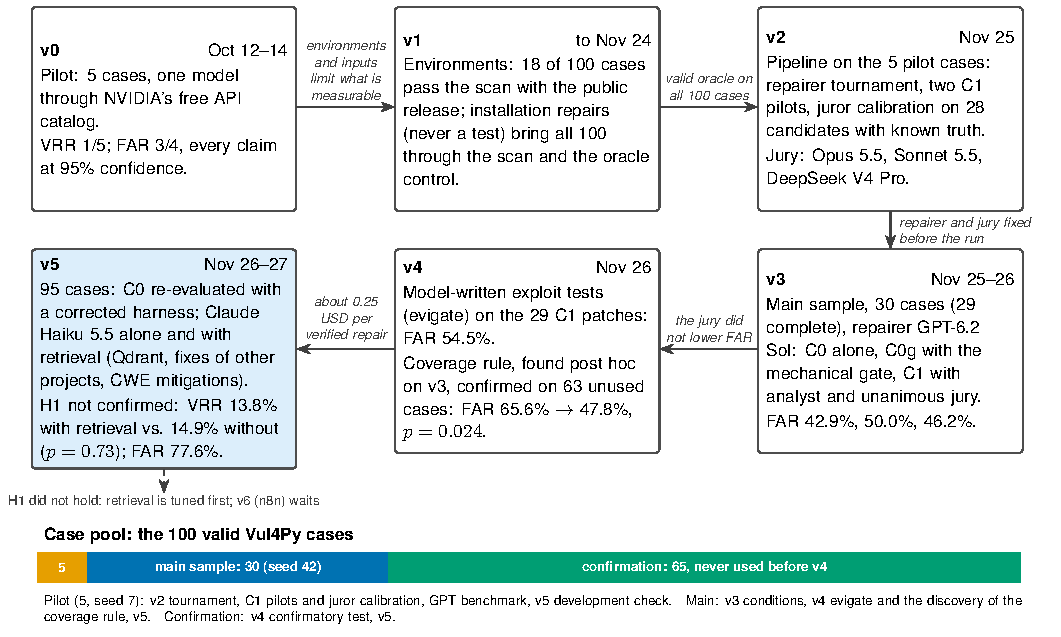
\includegraphics[width=\linewidth]{figures/fig_study_flow.pdf}
\end{adjustwidth}
\caption{Study flow. Each box gives what a version ran and its main result; the arrows give the reason for the next version. The bar at the bottom shows how the 100 valid cases were split and which versions used each part. Drawn from the TikZ source \texttt{figures/fig\_study\_flow.tex}.\label{fig:flow}}
\end{figure}

\subsection{Environment Validation (v1)}\label{sec:env}

A case is usable only if its oracle is valid on the machine that runs the experiments. Two checks decide this. The \emph{scan} installs the case and runs its tests with Vul4Py's own scripts. The \emph{oracle control} then requires that the functional tests pass on the unpatched vulnerable version, that the exploit tests fail on it, and that the upstream fix passes both; it runs through the same harness as the candidate patches, once per case and evaluation session. With the public release, only 18 of the 100 cases passed the first scan in a sandbox of the size of the instance. Table~\ref{tab:repairs} lists the problems found and the repairs. Every repair changes how a case is installed or which tests run, never a test or what it expects, and each one is recorded with its reason in \texttt{code/dataset/meta\_overrides/<case>.json} (91 files) or \texttt{code/dataset/test\_overrides/} (14 cases). Per case, the levels were applied in the order of the table, each only where the previous ones were not enough.

\begin{table}[H]
\caption{Installation repairs. Cases: number of the 91 override files whose note records the repair (a case can have several). The harness repairs apply to every case.\label{tab:repairs}}
\begin{adjustwidth}{-\extralength}{0cm}
\footnotesize
\begin{tabularx}{\fulllength}{@{}XXlr@{}}
\toprule
\textbf{Problem in the public release} & \textbf{Repair} & \textbf{Tag} & \textbf{Cases} \\
\midrule
\texttt{pip install -e .} misses the test dependencies & Extras, requirements files, pytest plugins and packages imported by the tests and by the fixed code & \texttt{doctor:deps} & 14 \\
Every case runs on Python 3.11 with 2026 libraries, while the fixes date from 2017--2025 & Newest Python the project supported at the fix date and every dependency resolved as of the fix date plus 30 days (\texttt{uv --exclude-newer}); kept only where it did not make the case worse & \texttt{doctor:era} & 63 \\
Suites that hang until the 900~s limit & Per-test timeouts & \texttt{timeouts} & 8 \\
Tests that fail even with the upstream fix (environment noise) & Vul4Py's own automatic deselection, with two fixes: node identifiers of private and nested test classes, and exploit tests that fail only for lack of network are never deselected & \texttt{auto\_skip} & 65 \\
Old functional tests that assert the vulnerable behaviour, so that even the upstream fix ``breaks'' functionality & Deselect exactly those tests & \texttt{oracle\_repair} & 26 \\
Functional tests that fail only on the vulnerable version and cannot separate a broken patch from a good one & Deselect them (single tests, at most 10 per case) & \texttt{vuln\_only} & 3 \\
Test files that abort or block the whole session, and per-project problems & Fixed case by case (32 tagged, 3 described in prose) & \texttt{manual} & 35 \\
PyTorch wheels of more than 6~GB & CPU-only wheels at the validated version & \texttt{torch\_cpu} & 6 \\
The harness deletes compiled products of the install; fixes outside \texttt{.py} files; commits reachable only by SHA; too many open files & Snapshot and restore of install products; every non-test code file of the fix in context and reference, rebuild after C or Rust patches; fetch by SHA; raised open-files limit & harness & all \\
\bottomrule
\end{tabularx}
\end{adjustwidth}
\end{table}

\subsection{Models, Context and the Multi-Model Pipeline}\label{sec:pipeline}

Table~\ref{tab:models} lists the models, their roles, their reasoning effort and their list prices. OpenAI and DeepSeek models were called through their APIs. Claude models were called through the Claude Code command-line client with the author's Claude subscription (one fresh session per call, no tools, the role's system prompt replacing the client's own, and the effort set from the configuration); these calls are not billed per call, and their cost is reported at the equivalent API list price.

\begin{table}[H]
\caption{Models, roles, reasoning effort and list prices (USD per million input/output tokens, \texttt{code/models.json}). DeepSeek prices are peak-hour prices; Haiku 5.5 costs 0.50/2.50 above 100k prompt tokens. Identifiers as in \texttt{code/models.json} (for example \texttt{openai:gpt-6.2-sol}, \texttt{claudecode:claude-opus-5-5}, \texttt{deepseek:deepseek-v4-pro}); every call of v2--v5 was made between 25 and 27 November 2026, those of v0 between 12 and 14 October 2026.\label{tab:models}}
\begin{adjustwidth}{-\extralength}{0cm}
\footnotesize
\begin{tabularx}{\fulllength}{@{}llXlr@{}}
\toprule
\textbf{Model} & \textbf{Access} & \textbf{Roles in this study} & \textbf{Effort} & \textbf{Price in/out} \\
\midrule
GPT-6.2 Sol & OpenAI API & Repairer (v2--v4); GPT benchmark & high & 2.00/10.00 \\
GPT-5.4 mini & OpenAI API & Repairer in the tournament and the first C1 pilot & high & 0.75/4.50 \\
GPT-6 Luna & OpenAI API & Analyst (C1); juror (first C1 pilot); calibration v1; GPT benchmark & medium & 0.10/0.50 \\
GPT-6.1 Sol & OpenAI API & Juror (first C1 pilot); calibration v1 & high & 2.00/10.00 \\
GPT-6.1 Terra & OpenAI API & Juror (first C1 pilot); calibration v1; GPT benchmark & medium & 1.00/5.00 \\
GPT-6.2 Astra & OpenAI API & Calibration v1; GPT benchmark & high & 8.00/40.00 \\
Claude Opus 5.5 & Claude Code (plan) & Juror (C1); calibration v2; attacker of evigate (effort high) & medium & 4.00/20.00 \\
Claude Sonnet 5.5 & Claude Code (plan) & Juror (C1); calibration v2 & medium & 2.00/10.00 \\
Claude Haiku 5.5 & Claude Code (plan) & Calibration v2; repairer (v5) & high & 0.10/0.50 \\
DeepSeek V4 Pro & DeepSeek API & Juror (C1); calibration v2 & high & 1.32/3.96 \\
DeepSeek Flash & DeepSeek API & Calibration v2 & high & 0.30/1.20 \\
laguna-xs-2.1 & NVIDIA API catalog & Repairer (v0) & -- & free \\
\bottomrule
\end{tabularx}
\end{adjustwidth}
\end{table}

\textbf{Context.} Every model received the same context: the vulnerable versions of the files that the upstream fix changed, library code first, and a hint with the line ranges of the vulnerability, as in the direct-prompting protocol of the Vul4Py paper~\cite{Bui2026Vul4pyBenchmarkingAutomated}. The code budget was 40\% of the smallest context window in the run; in the main runs every case fitted whole.

\textbf{Pipeline (condition C1).} Figure~\ref{fig:pipeline} shows the pipeline. An analyst describes the structure and data flow of the code; every statement must quote the code, and quotes that do not exist in it are dropped. The repairer writes a diagnosis with quoted evidence, a unified diff, a claim and a confidence. A mechanical gate checks, without running any test, that the patch applies the way Vul4Py applies patches, touches only files shown to the model, compiles, is not a no-op and is not oversized; a failing patch goes back to the repairer with the failure text, at most twice. A jury of three models from families other than the repairer's (Claude Opus 5.5, Claude Sonnet 5.5 and DeepSeek V4 Pro, chosen in v2) then votes on the candidate patches, each juror receiving them in its own shuffled order. If the vote is not unanimous, a debate round follows in which each juror sees the others' arguments, with their citations marked as verified or not, and votes again; if it is still split, the author of the leading patch revises it against the critiques, and the revision goes through the gate and the jury again. A unanimous verdict that the patch fixes the vulnerability is the claim of the system; without unanimity the system abstains and the leading patch is still evaluated. The code also supports several repairers with cross-examination and merging of equivalent patches; the main runs used a single repairer, so these steps did not run there. Condition C0 is the repairer alone with its own claim, and C0g adds only the gate.

\begin{figure}[H]
\begin{adjustwidth}{-\extralength}{0cm}
\centering
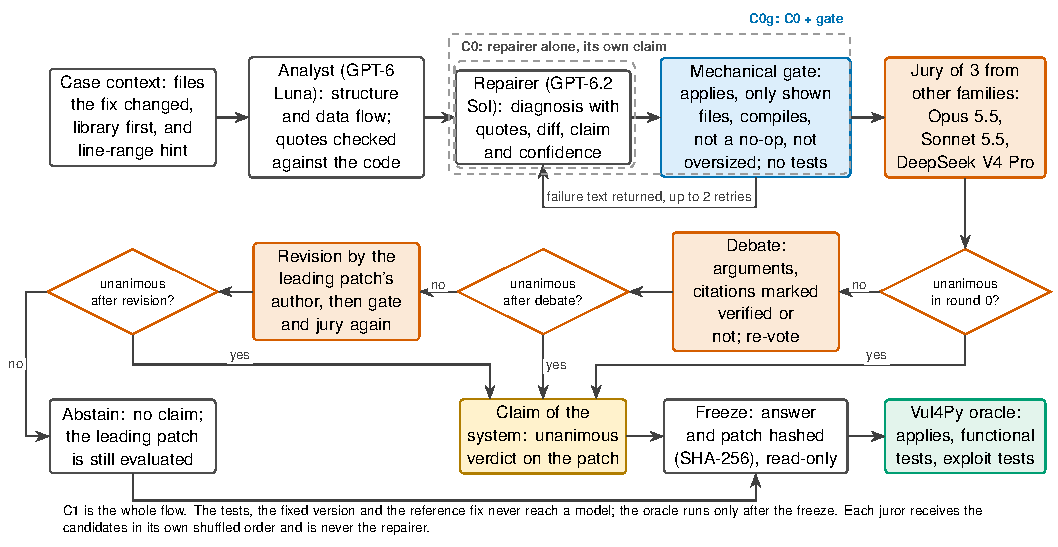
\includegraphics[width=\linewidth]{figures/fig_pipeline_c1.pdf}
\end{adjustwidth}
\caption{Multi-model pipeline (condition C1). Dashed frames mark the parts that form conditions C0 and C0g. Drawn from the TikZ source \texttt{figures/fig\_pipeline\_c1.tex}.\label{fig:pipeline}}
\end{figure}

\subsection{Pilot, Tournament and Juror Calibration (v2)}\label{sec:calib}

On the 5 pilot cases, two candidate repairers (GPT-6.2 Sol and GPT-5.4 mini) repaired alone, and two pilots of C1 ran end to end: the first with both repairers and a jury of GPT models (GPT-6.1 Sol, GPT-6.1 Terra and GPT-6 Luna), the second with GPT-6.2 Sol and the cross-family jury. After these runs, four GPT models also repaired the pilot cases through the Codex client (the GPT benchmark of v3). The first attempt at the main run, with a jury of GPT models, stopped when the OpenAI credit provided for the course ran out (25 November, 11:41~UTC); its outputs were archived and excluded.

Candidate jurors were calibrated on candidates whose truth was known: for each pilot case, the upstream fix ($V=1$), a decoy that compiles and changes nothing relevant ($V=0$), and the real patches of the pilot that applied, with their oracle verdicts. Calibration v2 used 28 candidates per model (13 correct, 15 wrong); calibration v1, with GPT models, used 23. Each candidate juror judged them as in the pipeline, and its stated confidence was scored by the area under the ROC curve (AUROC), sensitivity, specificity and the Brier score~\cite{Brier1950VerificationOfForecasts}. The rule fixed in \texttt{decisiones\_v2} took the three candidates with the highest AUROC with at least one per provider (Claude and DeepSeek), and a candidate that refused in two or more of the five calibration calls would have been excluded (none refused).

\subsection{Conditions and Claim Rules (v3)}\label{sec:conditions}

On the main sample, C0, C0g and C1 ran with GPT-6.2 Sol (effort high) as the repairer and GPT-6 Luna as the analyst of C1; C0 and C0g ran under \texttt{decisiones\_v1} and C1 under \texttt{decisiones\_v2}. The three conditions shared one oracle control per case. The primary claim of C1 is the unanimous jury. Because every vote is frozen, other claim rules can be computed from the same records without changing the protocol: the repairer's own claim, the first juror, \emph{consensus} (the repairer claims and a majority of the jury accepts), \emph{majority}, a \emph{confident majority} (a majority accepts with mean confidence of at least $\tau=0.8$, fixed beforehand; column \texttt{D\_gate} in the data), \emph{pre-revision} (unanimity in a round before the first revision, judged on the initial patch) and \emph{independent} (unanimity in round 0, before any debate, judged on the initial patch). The primary rule and $\tau$ were fixed in \texttt{decisiones\_v1}, pre-revision was its secondary analysis, and independent was added as exploratory after the second C1 pilot and before the main C1 run; the other rules are descriptive.

\subsection{Executable Evidence (v4, evigate)}\label{sec:evigate}

evigate is a general tool, written for this project, that claims ``fixed'' only with executable evidence. For each of the 29 C1 patches of the main sample, a blind attacker (Claude Opus 5.5, effort high, at most 120 turns and 30~min per session) reads a report with the same location hint and the vulnerable code, never the patch, and writes attack tests that must fail on the original code in two of two runs. A verifier with no model runs them in Docker (read-only root, no capabilities, 3~GB of memory, 1.5 CPUs, no network for the tests) and requires that they pass with the patch in two of two runs and that no project test that passed before fails with the patch; the attacker reaches only its model's API, through a proxy with an allowlist. Finally, a white-box attacker in a new session sees the patch and looks for a bypass. The claim is positive only if every step succeeds; otherwise the patch gets a status that names the failed step. The claims were compared, on the same patches, with the unanimous jury and the other rules of C1 (\texttt{decisiones\_v3}).

\subsection{Hint-Coverage Rule and Its Confirmation (v4)}\label{sec:coverage}

The hint coverage of a patch is the fraction of the hinted line ranges that the patch touches: a range $[a,b]$ counts as touched when a hunk of the patch in the same file overlaps $[a-3,b+3]$ in the line numbers of the original file. The \emph{coverage rule} keeps a positive claim only when the coverage is 1, and the secondary rule \emph{coverage75} when it is at least 0.75. The rule was found after looking at the main sample, so it was then tested on the 65 cases never used before, with C0 and the same configuration as in the main sample (\texttt{decisiones\_v4}). The primary test was a one-sided Fisher exact test~\cite{Fisher1922InterpretationOfChi} that, among the cases where the repairer claims a fix, the rule passes correct patches ($V=1$) more often than wrong ones; the hypothesis was to be confirmed if $p<0.05$ and the rule's FAR was lower than the repairer's on the same cases. By simulation, the power was 0.73 if the true effect equalled the one seen post hoc in C0, and 0.26 if it was half of it. The analysis was to be run once, when the run ended.

\subsection{Retrieval for a Cheaper Model (v5)}\label{sec:v5method}

The cost of C0 motivated v5: GPT-6.2 Sol cost about 0.25~USD per verified repair over the 92 complete cases of v3 and v4. v5 asks whether retrieval raises the VRR of Claude Haiku 5.5, whose list price is 20 times lower, on the 95 cases of the main sample and the confirmation (Figure~\ref{fig:v5}). Three arms run on the same cases and share one oracle control: C0, the frozen patches of GPT-6.2 Sol re-evaluated with the corrected harness and without model calls; M, Claude Haiku 5.5 (effort high) with the C0 prompt, byte for byte; and M+RAG, the same with a references section inserted before the source files.

\begin{figure}[H]
\begin{adjustwidth}{-\extralength}{0cm}
\centering
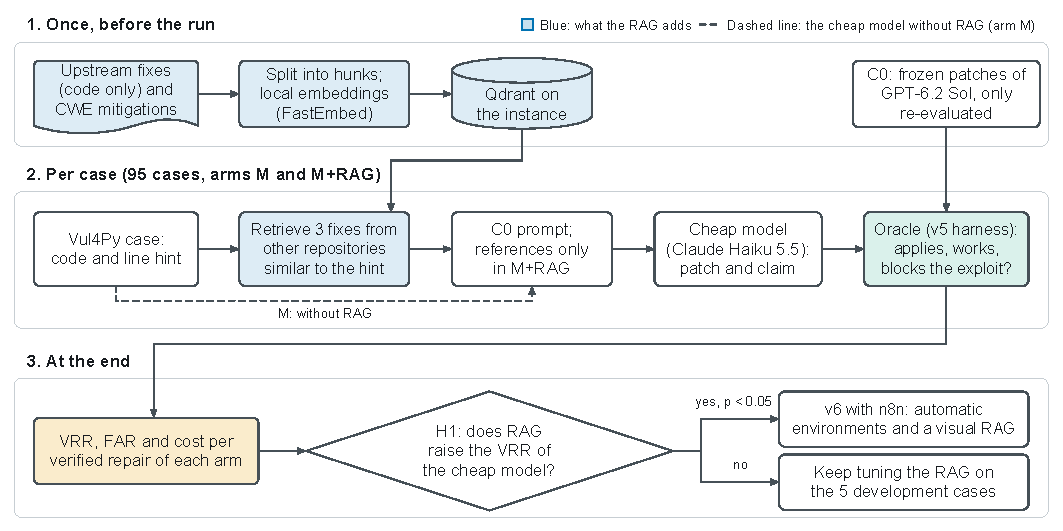
\includegraphics[width=\linewidth]{figures/fig_system_v5_chatgpt.pdf}
\end{adjustwidth}
\caption{System of v5: retrieval for a cheaper model. Blue marks what the retrieval step adds; the dashed line is arm M, the same model without retrieval. Drawn with ChatGPT (OpenAI) from a prompt that listed every component, label and connection (Section~\ref{sec:ai}); the TikZ source \texttt{figures/fig\_system\_v5.tex} draws the same diagram.\label{fig:v5}}
\end{figure}

\textbf{Harness.} Two options, off by default so that v1--v4 reproduce, address the two cases lost in v4. With \texttt{VUL4PY\_CLEAN\_ENV=1} the tests run without environment variables that hold keys (one project's tests had found an API key in the environment and called external services with it). With \texttt{VUL4PY\_FLAKE\_RERUN=2}, when one to three functional tests fail the suite is rerun up to twice and only a test that fails in every run counts as failed; exploit tests are never rerun. This addresses flaky tests~\cite{Luo2014EmpiricalAnalysisFlaky}, such as a client test that waited 5~s for a refused local connection in a case whose fix does not touch that code.

\textbf{Retrieval (RAG-R v1).} The knowledge base holds one chunk per hunk of the upstream fixes of the 100 cases (code files only, with 10 lines of vulnerable context; 913 chunks), each with its case, repository and CWE identifiers, taken from OSV~\cite{OpenSSF2026OsvSchema} or the GitHub advisory database (98 of 100 cases have at least one), and the mitigations of those CWEs from the MITRE CWE list, version 5.0~\cite{MITRE2026CweList}. Chunks are embedded locally on the CPU with FastEmbed~\cite{Qdrant2026FastEmbed} and the model \texttt{jina-embeddings-v2-base-code}~\cite{Gunther2023JinaEmbeddings2} (768 dimensions) and stored in Qdrant in local mode on the instance~\cite{Qdrant2026QdrantClient} (cosine distance), so that neither the code nor the fixes leave the instance. The query is the hinted code that the model already sees, with 20 lines of context. The search keeps the 40 nearest chunks from other repositories, so that neither the case's own fix nor the fixes of its project can be retrieved, takes the best chunk per source case and the top 3 cases, and adds the guidance of up to two CWEs of those cases, within 3000 tokens. The section tells the model that these are fixes of other projects that may not apply. For each case, a leakage audit compares every retrieved example with the case's own fix (difflib ratio on changed lines) and flags the case at 0.5 or more; H1 is also reported without flagged cases. The manifest of the knowledge base, with the SHA-256 of every part, was frozen in \texttt{decisiones\_v5}.

\textbf{Hypotheses.} The primary hypothesis H1 is VRR(M+RAG)~$>$~VRR(M) on the cases complete in both arms, tested with a one-sided exact McNemar test~\cite{McNemar1947NoteOnThe} at $\alpha=0.05$. Its exact power with 94 cases was 0.65 if retrieval wins in 15\% of the cases and loses in 5\%, and 0.20 for a net gain of 4 points. The secondary estimates are: the cost per verified repair of M+RAG relative to C0, as a ratio with a paired bootstrap interval~\cite{Efron1979BootstrapMethods} (10,000 resamples of cases, seed 2026, list prices); the difference VRR(M+RAG)~$-$~VRR(C0) with Newcombe's interval for paired data~\cite{Newcombe1998ImprovedConfidenceIntervals}; FAR and safe yield of each arm; the coverage rule in M and M+RAG, to see whether it replicates with another model family; and the C0 verdicts that change with the corrected harness. A development check on the 5 pilot cases, not part of the analysis, verified that Haiku produces applicable patches and that retrieval works. The rule for the next version was also fixed beforehand: v6 (automatic environment repair and the retrieval step as an n8n workflow) proceeds only if H1 is confirmed.

\subsection{Calls, Tokens, Time and Cost}\label{sec:cost}

Every model call was recorded with its model, role, input and output tokens, latency, HTTP attempts and status, and its list-price cost, computed as tokens times the prices of Table~\ref{tab:models} (files \texttt{results/logs/calls/*.csv}). For Claude calls through the subscription, the client's own cost report is also recorded; it equals the list price with every input token counted at twice the input price, so it is higher than the list price (for example 20.47 against 11.93~USD for the Opus juror calls). Tables and figures use the list price for every provider so that providers are compared on the same basis. The juror calibration of v2 recorded totals per model rather than per call.

\subsection{Statistical Analysis}\label{sec:stats}

Proportions are reported with 95\% Wilson score intervals~\cite{Wilson1927ProbableInferenceLaw,Brown2001IntervalEstimationFor}. Claims of two rules on the same attempts are compared with the exact McNemar test on the discordant pairs (two-sided, descriptive unless stated otherwise). The confirmatory tests are the one-sided Fisher test of v4 and the one-sided exact McNemar test of H1 in v5; every other test is descriptive or exploratory, and no correction for multiple comparisons is applied to them. The analyses are computed by \texttt{fa\_metrics.py}, \texttt{confirm\_v4.py} and \texttt{confirm\_v5.py} from the frozen records.

\subsection{Use of Generative AI}\label{sec:ai}

LLMs are the object of this study: for v0 and for every case of v2--v4 and the v5 development check that went through the pipeline, the answers of every model, the patches, their evaluation and the record of every call (tokens, latency, cost and the SHA-256 of its prompt) are released with the paper. In addition, the author used Claude Opus 5.5 (Anthropic) as an assistant to write and review the scripts of the study, to organise the repository, to write the TikZ code of Figures~\ref{fig:flow} and~\ref{fig:pipeline} from components and connections specified by the author, to write the prompts for Figures~\ref{fig:v5} and~\ref{fig:v6}, and to draft and edit the text of this manuscript. Figures~\ref{fig:v5} and~\ref{fig:v6} were drawn with ChatGPT (OpenAI, model GPT-6.2 Sol) from those prompts, and every label and connection was checked against the decisions files. All numbers were computed by the released scripts from the frozen records of the runs, every reference was checked in a scholarly source, and the author reviewed the output and takes full responsibility for the content.

%-----------------------------------------------------------------------------------------------
\section{Results}\label{sec:results}

\subsection{Environments (v1)}\label{sec:resenv}

With the public release, 18 of the 100 cases passed the first scan. With the repairs of Table~\ref{tab:repairs}, the scan on the instance passed 86 cases in the first build round, 98 in the second, 99 in the third to fifth and 100 in the sixth, and all 100 cases passed the oracle control: their functional tests pass unpatched, their exploit tests fail unpatched, and the upstream fix passes both (Figure~\ref{fig:env}). The most frequent repairs were the automatic deselection of tests that fail even with the upstream fix (65 cases) and the era-matched Python and dependencies (63 cases; 54 override files also set the Python version). Twenty-six cases had functional tests that assert the vulnerable behaviour, so that the upstream fix itself would have been counted as breaking functionality.

\begin{figure}[H]
\begin{adjustwidth}{-\extralength}{0cm}
\centering
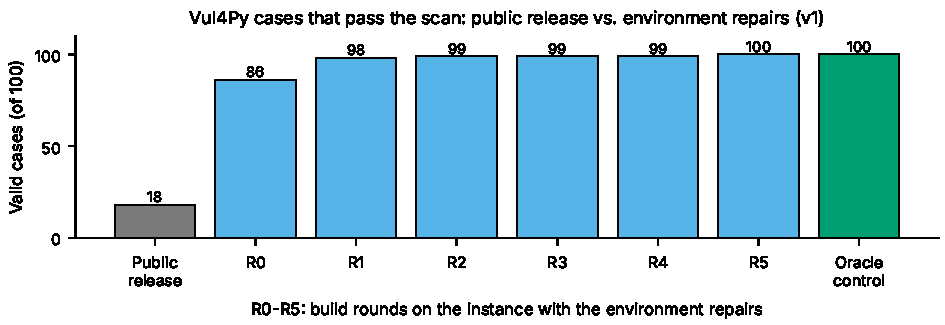
\includegraphics[width=\linewidth]{figures/fig_environment.pdf}
\end{adjustwidth}
\caption{Cases that pass the scan with the public release (in a sandbox of the size of the instance) and after each build round on the instance (R0--R5), and cases that pass the oracle control; only the build rounds are joined, since they form one series. Drawn by \texttt{results/figures/make\_figures.py} from \texttt{experiments/v1\_environment/scan\_report\_round*.tsv} and \texttt{oracle\_report.tsv} (checked against \texttt{prereg/oracle\_valid.txt}); the public-release count is the one recorded in \texttt{code/docs/README\_multiagent.md}.\label{fig:env}}
\end{figure}

\subsection{Pilot-Scale Comparisons (v2 and v3)}\label{sec:respilot}

Table~\ref{tab:pilot} and Figure~\ref{fig:pilotfig} give every comparison run on the five pilot cases. GPT-6.2 Sol verified three repairs and GPT-5.4 mini one, and GPT-5.4 mini made four false claims out of five; GPT-6.2 Sol was kept as the only repairer of the main runs. In the first C1 pilot the unanimous jury of GPT models removed one of the two false claims of the repairer and kept one; in the second, the cross-family jury claimed all five patches, including both wrong ones. In that pilot the jury had not accepted either wrong patch in round 0; one was accepted after the debate and the other after the revision. Through the Codex client, GPT-6.2 Astra and GPT-6.2 Sol each verified three repairs, GPT-6.1 Terra one and GPT-6 Luna none (four of its answers had an empty patch).

\begin{table}[H]
\caption{Comparisons on the five pilot cases. Claims are the positive claims of the system (the repairer's own claim, or the unanimous jury in C1). The GPT benchmark recorded verdicts only.\label{tab:pilot}}
\begin{adjustwidth}{-\extralength}{0cm}
\footnotesize
\begin{tabularx}{\fulllength}{@{}lXlcc@{}}
\toprule
\textbf{Run} & \textbf{Configuration} & \textbf{VRR} & \textbf{Claims} & \textbf{False assurances} \\
\midrule
Tournament & GPT-6.2 Sol alone & 3/5 & 5 & 2 \\
Tournament & GPT-5.4 mini alone & 1/5 & 5 & 4 \\
C1 pilot 1 & Repairers GPT-6.2 Sol and GPT-5.4 mini; jury GPT-6.1 Sol, GPT-6.1 Terra, GPT-6 Luna & 3/5 & 4 & 1 \\
C1 pilot 2 & Repairer GPT-6.2 Sol; jury Claude Opus 5.5, Claude Sonnet 5.5, DeepSeek V4 Pro & 3/5 & 5 & 2 \\
GPT benchmark & GPT-6 Luna / GPT-6.1 Terra / GPT-6.2 Astra / GPT-6.2 Sol / GPT-6.2 Sol with trimmed context (Codex) & 0/5, 1/5, 3/5, 3/5, 3/5 & -- & -- \\
\bottomrule
\end{tabularx}
\end{adjustwidth}
\end{table}

\begin{figure}[H]
\begin{adjustwidth}{-\extralength}{0cm}
\centering
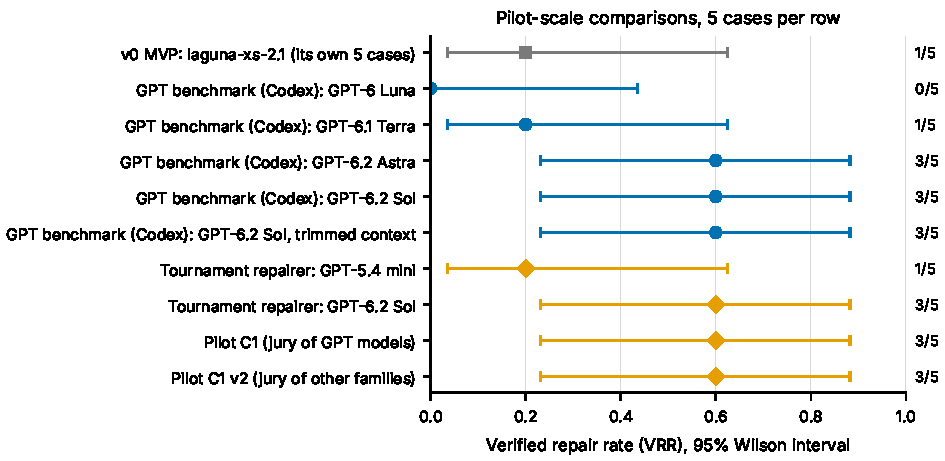
\includegraphics[width=\linewidth]{figures/fig_pilot_benchmarks.pdf}
\end{adjustwidth}
\caption{VRR with 95\% Wilson intervals of every comparison run on five cases: the v0 pilot on its own five cases, the GPT benchmark, the tournament repairers and the two C1 pilots. Drawn by \texttt{results/figures/make\_figures.py} from \texttt{experiments/v0\_mvp/results.csv}, \texttt{experiments/v2\_pilot\_tournament/results.csv} and \texttt{experiments/v3\_main/gpt\_benchmark/gpt\_benchmark\_verdicts.csv}.\label{fig:pilotfig}}
\end{figure}

\subsection{Juror Calibration (v2)}\label{sec:rescalib}

Table~\ref{tab:calib} and Figure~\ref{fig:calib} give the calibration of the candidate jurors. In calibration v2 the confidence of the three Claude models separated correct from wrong candidates best (AUROC 0.900--0.913), followed by DeepSeek V4 Pro (0.838), which had the highest specificity (0.933), and DeepSeek Flash (0.744). By the rule fixed beforehand, the jury was Claude Opus 5.5, Claude Sonnet 5.5 and DeepSeek V4 Pro; Claude Haiku 5.5 was left out by the one-per-provider condition. No candidate refused. The GPT models of calibration v1 reached AUROC values between 0.672 and 0.800. The calibration cost 2.14~USD at list price (2.64~USD with the client's own report for the Claude calls).

\begin{table}[H]
\caption{Calibration of candidate jurors on candidates with known truth: AUROC of the stated confidence, sensitivity (correct candidates accepted), specificity (wrong candidates rejected) and Brier score. Cost: list price of the five calibration calls.\label{tab:calib}}
\begin{adjustwidth}{-\extralength}{0cm}
\footnotesize
\begin{tabularx}{\fulllength}{@{}Xlccccc@{}}
\toprule
\textbf{Candidate juror} & \textbf{Calibration} & \textbf{AUROC} & \textbf{Sensitivity} & \textbf{Specificity} & \textbf{Brier} & \textbf{Cost (USD)} \\
\midrule
Claude Opus 5.5 (selected) & v2, 28 candidates & 0.913 & 0.846 & 0.667 & 0.126 & 0.68 \\
Claude Sonnet 5.5 (selected) & v2, 28 candidates & 0.905 & 0.846 & 0.733 & 0.145 & 0.30 \\
Claude Haiku 5.5 & v2, 28 candidates & 0.900 & 0.769 & 0.733 & 0.155 & 0.08 \\
DeepSeek V4 Pro (selected) & v2, 28 candidates & 0.838 & 0.846 & 0.933 & 0.150 & 0.81 \\
DeepSeek Flash & v2, 28 candidates & 0.744 & 0.846 & 0.867 & 0.214 & 0.28 \\
GPT-6.1 Sol & v1, 23 candidates & 0.800 & 0.600 & 0.778 & 0.245 & -- \\
GPT-6.1 Terra & v1, 23 candidates & 0.711 & 0.600 & 0.833 & 0.201 & -- \\
GPT-6.2 Astra & v1, 23 candidates & 0.700 & 0.600 & 0.833 & 0.215 & -- \\
GPT-6 Luna & v1, 23 candidates & 0.672 & 0.800 & 0.778 & 0.421 & -- \\
\bottomrule
\end{tabularx}
\end{adjustwidth}
\end{table}

\begin{figure}[H]
\begin{adjustwidth}{-\extralength}{0cm}
\centering
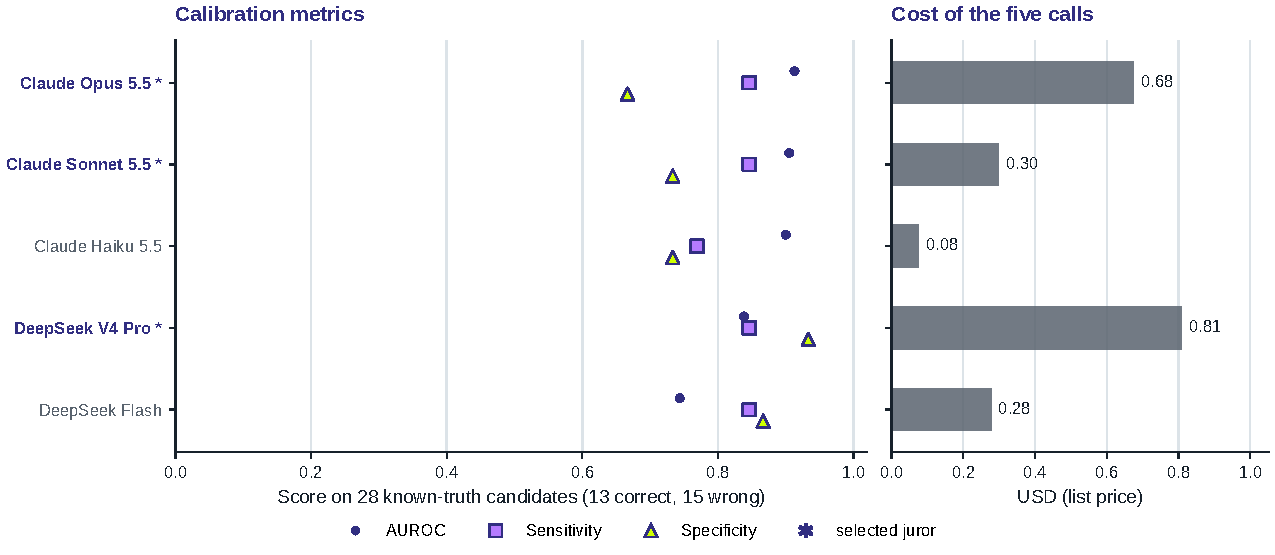
\includegraphics[width=\linewidth]{figures/fig_jury_calibration.pdf}
\end{adjustwidth}
\caption{Calibration v2. Left: AUROC of the stated confidence, sensitivity and specificity of each candidate juror on 28 candidates with known truth (13 correct, 15 wrong). Right: list-price cost of its five calls. Asterisks mark the three selected jurors. Drawn by \texttt{results/figures/make\_figures.py} from \texttt{experiments/v2\_pilot\_tournament/judge\_calibration\_v2/} (summary and token use), the prices in \texttt{code/models.json} and the jury in \texttt{prereg/decisiones\_v2.txt}.\label{fig:calib}}
\end{figure}

\subsection{Main Sample (v3)}\label{sec:resmain}

Of the 30 cases of the main sample, 29 were complete in all three conditions: the exploit test of orjson CVE-2024-27454 kills the test process with a segmentation fault, so the case was excluded in every condition. Table~\ref{tab:main} and Figure~\ref{fig:main} give the results (RQ1, RQ2). The repairer alone verified 16 of 29 repairs, and 12 of its 28 positive claims were false (FAR 42.9\%). Adding the mechanical gate did not lower FAR (50.0\%), and neither did the analyst and the unanimous jury of C1 (46.2\%); both had two fewer verified repairs than C0, a difference of two cases out of 29. With 26 to 28 positive claims per condition, each FAR interval spans about 35 percentage points, so these data show no reduction but cannot exclude a moderate one. Most unverified patches applied and kept the functional tests passing but failed the exploit tests: 12 of 13 in C0, 14 of 15 in C0g and 13 of 15 in C1. On the 63 complete cases of the confirmation run (v4), the same repairer verified 34.9\% of the repairs and 65.6\% of its positive claims were false, with the same pattern (34 of the 41 unverified patches).

\begin{table}[H]
\caption{Results on the main sample (v3) and C0 on the confirmation cases (v4). Claims: positive claims of the system. Last two columns: unverified patches that did not apply or broke the functional tests, and patches that passed the functional tests but failed the exploit tests. Intervals are 95\% Wilson intervals.\label{tab:main}}
\begin{adjustwidth}{-\extralength}{0cm}
\footnotesize
\begin{tabularx}{\fulllength}{@{}Xccccccc@{}}
\toprule
\textbf{Condition} & \textbf{N} & \textbf{VRR (95\% CI)} & \textbf{Claims} & \textbf{FAR (95\% CI)} & \textbf{Safe yield} & \textbf{Broke} & \textbf{Exploit fails} \\
\midrule
C0: repairer alone & 29 & 16/29 = 55.2\% (37.5--71.6) & 28 & 12/28 = 42.9\% (26.5--60.9) & 55.2\% & 1 & 12 \\
C0g: + mechanical gate & 29 & 14/29 = 48.3\% (31.4--65.6) & 28 & 14/28 = 50.0\% (32.6--67.4) & 48.3\% & 1 & 14 \\
C1: + analyst and unanimous jury & 29 & 14/29 = 48.3\% (31.4--65.6) & 26 & 12/26 = 46.2\% (28.8--64.5) & 48.3\% & 2 & 13 \\
C0, confirmation cases (v4) & 63 & 22/63 = 34.9\% (24.3--47.2) & 61 & 40/61 = 65.6\% (53.0--76.3) & 33.3\% & 7 & 34 \\
\bottomrule
\end{tabularx}
\end{adjustwidth}
\end{table}

\begin{figure}[H]
\begin{adjustwidth}{-\extralength}{0cm}
\centering
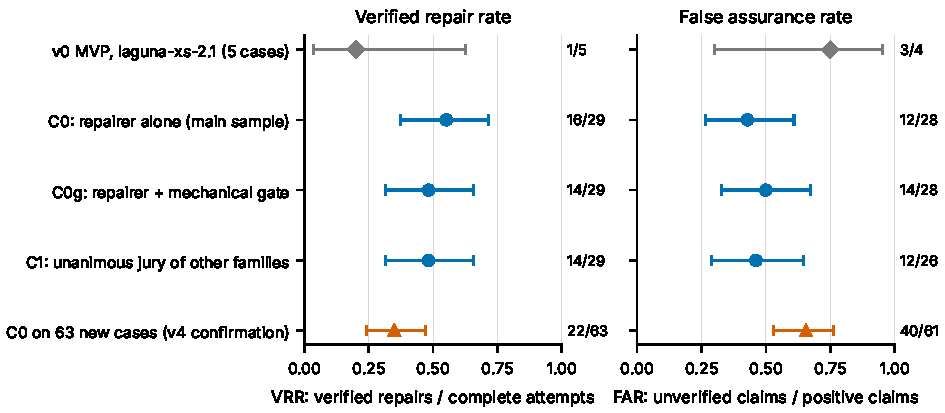
\includegraphics[width=\linewidth]{figures/fig_main_vrr_far.pdf}
\end{adjustwidth}
\caption{VRR and FAR with 95\% Wilson intervals: the v0 pilot, the three conditions of the main sample and C0 on the 63 confirmation cases. Drawn by \texttt{results/figures/make\_figures.py} from \texttt{experiments/v0\_mvp/results.csv}, \texttt{experiments/v3\_main/results.csv} and \texttt{experiments/v4\_evigate\_confirmation/confirm/results.csv}.\label{fig:main}}
\end{figure}

\subsection{Claim Rules and the Jury Protocol (v3)}\label{sec:resrules}

Table~\ref{tab:rules} applies every claim rule to the same 29 C1 attempts. The unanimous jury caught one false claim of the repairer (McNemar $p=1.000$). Only the confident majority lowered FAR noticeably, from 48.1\% to 36.8\% ($p=0.031$ on false assurances), and it did so by claiming 19 instead of 27 patches, which lowered the safe yield from 48.3\% to 41.4\%. The independent vote in round 0, before any debate, claimed 21 patches with FAR 42.9\%; debate and revision added claims, and with them false ones. Table~\ref{tab:protocols} gives the behaviour of the protocol. C1 abstained in 3 of the 29 cases; 21 cases were resolved by the independent vote, 5 after the debate and none after a revision (a revision reached unanimity only in the excluded orjson case). The gate rejected few patch versions, and most of them were repaired after its feedback. Quotes of code that does not exist were rare (1 of 1535 citations in C1), and no model refused. In every condition, whenever some candidate patch was correct, the selected one was correct.

\begin{table}[H]
\caption{Claim rules on the 29 complete attempts of C1 and the claims of evigate on the same patches. McNemar: exact test on false assurances against the repairer's claim (for evigate, against the unanimous jury).\label{tab:rules}}
\begin{adjustwidth}{-\extralength}{0cm}
\footnotesize
\begin{tabularx}{\fulllength}{@{}Xccccc@{}}
\toprule
\textbf{Rule} & \textbf{Claims} & \textbf{False assurances} & \textbf{FAR (95\% CI)} & \textbf{Safe yield} & \textbf{McNemar $p$} \\
\midrule
Repairer's own claim & 27 & 13 & 48.1\% (30.7--66.0) & 48.3\% & -- \\
First juror & 27 & 13 & 48.1\% (30.7--66.0) & 48.3\% & 1.000 \\
Consensus (repairer and majority) & 26 & 12 & 46.2\% (28.8--64.5) & 48.3\% & 1.000 \\
Majority & 27 & 13 & 48.1\% (30.7--66.0) & 48.3\% & 1.000 \\
Unanimous jury (primary) & 26 & 12 & 46.2\% (28.8--64.5) & 48.3\% & 1.000 \\
Confident majority (mean confidence $\geq 0.8$) & 19 & 7 & 36.8\% (19.1--59.0) & 41.4\% & 0.031 \\
Pre-revision (initial patch) & 25 & 11 & 44.0\% (26.7--62.9) & 48.3\% & 0.500 \\
Independent vote in round 0 (initial patch) & 21 & 9 & 42.9\% (24.5--63.5) & 41.4\% & 0.125 \\
evigate, executable evidence (v4) & 11 & 6 & 54.5\% (28.0--78.7) & 17.2\% & 0.031 \\
\bottomrule
\end{tabularx}
\end{adjustwidth}
\end{table}

\begin{table}[H]
\caption{Behaviour of the protocol in the three conditions of the main sample (29 complete attempts each; model calls and API time count all 30 attempted cases).\label{tab:protocols}}
\begin{adjustwidth}{-\extralength}{0cm}
\footnotesize
\begin{tabularx}{\fulllength}{@{}Xccc@{}}
\toprule
\textbf{Measure} & \textbf{C0} & \textbf{C0g} & \textbf{C1} \\
\midrule
Abstentions (no unanimous verdict) & -- & -- & 3 (10.3\%) \\
Resolved by independent vote / after debate / after revision & -- & -- & 21 / 5 / 0 \\
Patch versions rejected by the gate (repaired after its feedback) & -- & 3 (2) & 2 (2) \\
Quoted code that does not exist & 0 of 300 & 2 of 322 & 1 of 1535 \\
Refusals & 0 & 0 & 0 \\
Cases with a correct candidate / with the correct candidate selected & 16 / 16 & 14 / 14 & 14 / 14 \\
Model calls & 30 & 35 & 215 \\
Median API time per case (s) & 114 & 98 & 453 \\
\bottomrule
\end{tabularx}
\end{adjustwidth}
\end{table}

\subsection{Executable Evidence (v4)}\label{sec:resevigate}

evigate claimed 11 of the 29 C1 patches, and 6 of those 11 were wrong (FAR 54.5\%, Table~\ref{tab:rules}). Against the unanimous jury on the same patches it removed 6 false claims and added none ($p=0.031$), but it also lost 9 correct claims and gained none, so its safe yield fell to 17.2\%. Against the confident majority it removed 4 false claims, added 3, lost 8 correct claims and gained 1. Table~\ref{tab:evigate} shows why it did not separate correct from wrong patches: it verified 5 of the 14 correct patches and 6 of the 15 wrong ones, and its rejections of correct patches came from bypasses found by the white-box attacker (3), attack tests that the patch did not block (2), missing functional evidence (2), and failures to build the environment (1) or to reproduce the attack (1). In the six wrong patches it verified, the attack tests written from the report passed with the patch while the oracle did not verify it. The 29 patches took 5.75~h of tool time (median 656~s per patch).

\begin{table}[H]
\caption{Status assigned by evigate to the 29 C1 patches, by oracle verdict.\label{tab:evigate}}
\begin{adjustwidth}{-\extralength}{0cm}
\footnotesize
\begin{tabularx}{\fulllength}{@{}lXccc@{}}
\toprule
\textbf{Status} & \textbf{Meaning} & \textbf{Correct ($V=1$)} & \textbf{Wrong ($V=0$)} & \textbf{Total} \\
\midrule
verified & Attack tests reproduce on the original and pass with the patch; no regression; no bypass found (claim) & 5 & 6 & 11 \\
bypass & The white-box attacker found a bypass & 3 & 1 & 4 \\
not blocked & The reproduced attack still succeeds with the patch & 2 & 2 & 4 \\
no functional evidence & No project test passes on the original, so regressions cannot be checked & 2 & 2 & 4 \\
not reproduced & The attack tests do not fail on the original in two of two runs & 1 & 2 & 3 \\
environment failed & The environment of the case did not build & 1 & 1 & 2 \\
regression & A project test that passed on the original fails with the patch & 0 & 1 & 1 \\
\midrule
Total & & 14 & 15 & 29 \\
\bottomrule
\end{tabularx}
\end{adjustwidth}
\end{table}

\subsection{Hint-Coverage Rule: Discovery and Confirmation (v4)}\label{sec:rescov}

On the main sample, keeping a claim only when the patch touched every hinted line range lowered FAR in the three conditions (Table~\ref{tab:coverage}); the rule passed correct patches more often than wrong ones in all three, clearly only in C1 (9 of 14 against 2 of 13). Because the rule was chosen after seeing these data, it was then tested on the 65 unused cases (RQ3). Two of them were incomplete because of the environment: a tornado client test that timed out waiting for a refused local connection, in code that the fix does not touch, and smolagents tests that found an API key in the environment. On the 63 complete cases the rule passed 12 of the 21 correct claims and 11 of the 40 wrong ones (57.1\% against 27.5\%; one-sided Fisher $p=0.0237$; difference 0.30, 95\% CI 0.04--0.51, hybrid score interval~\cite{Newcombe1998IntervalEstimationIndependent}). FAR fell from 65.6\% to 47.8\% on the same cases, so the hypothesis was confirmed by both criteria fixed beforehand (Figure~\ref{fig:coverage}). The rule removed 29 false assurances and lost 9 correct claims, and the safe yield fell from 33.3\% to 19.0\%. The secondary rule coverage75 gave a similar FAR (48.1\%) with fewer correct claims lost (7). One deviation is reported: the confirmatory analysis was first run while 3 cases had no verdict yet ($N=60$, $p=0.022$); it was rerun when the run ended, as the decisions file requires, and the conclusion did not change.

\begin{table}[H]
\caption{Hint-coverage rule. Discovery: post hoc on the main sample (C1 with the repairer's claims). Confirmation: C0 on the 63 complete unused cases. Pass rates are the share of correct and of wrong claimed patches that the rule keeps; $p$: one-sided Fisher exact test.\label{tab:coverage}}
\begin{adjustwidth}{-\extralength}{0cm}
\footnotesize
\begin{tabularx}{\fulllength}{@{}Xccccc@{}}
\toprule
\textbf{Sample and rule} & \textbf{FAR of all claims} & \textbf{FAR with the rule} & \textbf{Pass rate correct} & \textbf{Pass rate wrong} & \textbf{$p$} \\
\midrule
Discovery, C0 & 12/28 = 42.9\% & 3/12 = 25.0\% & 9/16 & 3/12 & 0.102 \\
Discovery, C0g & 14/28 = 50.0\% & 5/13 = 38.5\% & 8/14 & 5/14 & 0.225 \\
Discovery, C1 & 13/27 = 48.1\% & 2/11 = 18.2\% & 9/14 & 2/13 & 0.013 \\
Confirmation, coverage (primary) & 40/61 = 65.6\% (53.0--76.3) & 11/23 = 47.8\% (29.2--67.0) & 12/21 & 11/40 & 0.024 \\
Confirmation, coverage75 & 40/61 = 65.6\% (53.0--76.3) & 13/27 = 48.1\% (30.7--66.0) & 14/21 & 13/40 & 0.011 \\
\bottomrule
\end{tabularx}
\end{adjustwidth}
\end{table}

\begin{figure}[H]
\centering
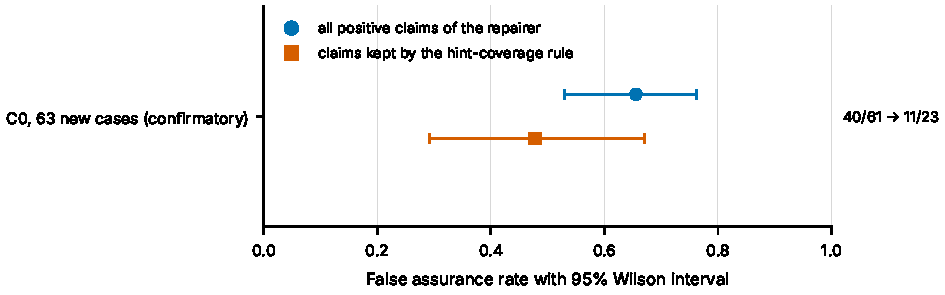
\includegraphics[width=\linewidth]{figures/fig_coverage_rule.pdf}
\caption{Confirmatory test of the hint-coverage rule: FAR with 95\% Wilson intervals of all positive claims of the repairer and of the claims kept by the rule, C0 on the 63 confirmation cases. Drawn by \texttt{results/figures/make\_figures.py} from \texttt{experiments/v4\_evigate\_confirmation/confirm/results.csv}.\label{fig:coverage}}
\end{figure}

\subsection{Retrieval for a Cheaper Model (v5)}\label{sec:resv5}

In the development check on the five pilot cases, which is not part of the analysis, Claude Haiku 5.5 answered every case in both arms without refusals, and only one of its five patches without retrieval did not apply or broke functionality, so it passed the feasibility gate (the threshold for switching models was three). Both arms verified 2 of 5 repairs with 2 false claims out of 4; the retrieval sections had between 585 and 1269 tokens and none was flagged by the leakage audit. The ten calls cost 0.124~USD at list price. Table~\ref{tab:v5} gives the main run. \pend{v5 main run: VRR, FAR, safe yield and cost of C0, M and M+RAG on the 95 cases; H1 with the exact one-sided McNemar test (discordant pairs and $p$); H1 without flagged cases; the cost-ratio bootstrap interval; the Newcombe interval of VRR(M+RAG) - VRR(C0); the coverage rule in M and M+RAG; the C0 verdicts that changed with the corrected harness}

\begin{table}[H]
\caption{Retrieval for a cheaper model. Development: the five pilot cases (not analysed). Main run: the 95 cases of the main sample and the confirmation. Cost at list price.\label{tab:v5}}
\begin{adjustwidth}{-\extralength}{0cm}
\footnotesize
\begin{tabularx}{\fulllength}{@{}Xcccccc@{}}
\toprule
\textbf{Arm} & \textbf{N} & \textbf{VRR} & \textbf{Claims} & \textbf{FAR} & \textbf{Cost (USD)} & \textbf{Per verified repair} \\
\midrule
Development, M (Haiku 5.5) & 5 & 2/5 & 4 & 2/4 & 0.059 & 0.029 \\
Development, M+RAG & 5 & 2/5 & 4 & 2/4 & 0.065 & 0.033 \\
\midrule
Main run, C0 (GPT-6.2 Sol, v5 harness) & \multicolumn{6}{l}{\pend{N, VRR, claims, FAR (Wilson CI) and cost when the run ends}} \\
Main run, M (Haiku 5.5) & \multicolumn{6}{l}{\pend{same columns}} \\
Main run, M+RAG & \multicolumn{6}{l}{\pend{same columns}} \\
\bottomrule
\end{tabularx}
\end{adjustwidth}
\end{table}

\subsection{Calls, Tokens, Time and Cost}\label{sec:rescost}

Tables~\ref{tab:costrun}--\ref{tab:costrepair} and Figures~\ref{fig:calls} and~\ref{fig:cost} give the accounting (RQ4). The runs of v2--v4 and the v5 development check made 497 model calls, including the 25 of the juror calibration, and cost 50.0~USD at list price. Most of it went to the main sample (34.40~USD), and within it to C1 (27.40~USD), whose jurors read the case and every candidate in each round: the Opus and Sonnet jurors averaged more than 41,000 input tokens per call. DeepSeek V4 Pro was the slowest model (median 193.6~s per call) and wrote the most output tokens per call, about 22,500. In cost per verified repair, C0 was the cheapest configuration of the main sample (0.21~USD), C0g cost 0.26~USD and C1 1.96~USD, 9.4 times as much as C0 for the same or fewer verified repairs and no lower FAR. On the confirmation cases C0 cost 0.28~USD per verified repair. \pend{v5: calls, tokens and cost of M and M+RAG on the 95 cases, and their cost per verified repair against C0}

\begin{table}[H]
\caption{Calls, tokens, summed call time and list-price cost per run. Client report: the cost that the Claude client reports for the Claude calls made through the subscription, which counts input tokens at twice the input price; the list price of the same calls is in parentheses.\label{tab:costrun}}
\begin{adjustwidth}{-\extralength}{0cm}
\footnotesize
\begin{tabularx}{\fulllength}{@{}Xrrrrrl@{}}
\toprule
\textbf{Run} & \textbf{Calls} & \textbf{Input tokens} & \textbf{Output tokens} & \textbf{Call time (h)} & \textbf{List price (USD)} & \textbf{Client report (USD)} \\
\midrule
v0 pilot (NVIDIA API catalog) & 5 & 18,989 & 845 & 0.23 & 0 (free) & -- \\
v2 tournament and C1 pilots & 117 & 1,283,730 & 986,284 & 2.35 & 7.22 & 2.48 (1.57) \\
v2 juror calibration & 25 & 349,054 & 572,872 & -- & 2.14 & 1.55 (1.05) \\
v3 main sample (C0, C0g, C1) & 280 & 8,105,924 & 2,356,785 & 6.87 & 34.40 & 27.60 (15.70) \\
v4 confirmation (C0) & 65 & 848,338 & 442,252 & 1.70 & 6.12 & -- \\
v5 development check & 10 & 138,975 & 220,165 & 0.24 & 0.12 & 0.14 (0.12) \\
v5 main run (M and M+RAG) & \multicolumn{6}{l}{\pend{calls, tokens, time and cost when the run ends}} \\
\bottomrule
\end{tabularx}
\end{adjustwidth}
\end{table}

\begin{table}[H]
\caption{Calls by model and role over every per-call record (v0, v2--v4 and the v5 development check; the 25 calibration calls are recorded as totals and not included). Latency: median seconds per call. In parentheses: the Claude client's own report. The rows do not add up exactly to the total because of rounding.\label{tab:costmodel}}
\begin{adjustwidth}{-\extralength}{0cm}
\footnotesize
\begin{tabularx}{\fulllength}{@{}Xlrrrrr@{}}
\toprule
\textbf{Model} & \textbf{Role} & \textbf{Calls} & \textbf{Input tokens} & \textbf{Output tokens} & \textbf{Latency (s)} & \textbf{List price (USD)} \\
\midrule
GPT-6.2 Sol & repairer & 193 & 3,361,372 & 1,336,030 & 91.7 & 20.08 \\
Claude Opus 5.5 & juror & 57 & 2,134,275 & 169,842 & 26.4 & 11.93 (20.47) \\
DeepSeek V4 Pro & juror & 57 & 1,406,726 & 1,284,226 & 193.6 & 6.94 \\
Claude Sonnet 5.5 & juror & 57 & 2,139,020 & 105,212 & 13.4 & 5.33 (9.61) \\
GPT-5.4 mini & repairer & 22 & 210,005 & 365,519 & 72.8 & 1.80 \\
GPT-6.1 Sol & juror & 12 & 132,328 & 81,999 & 111.0 & 1.08 \\
GPT-6.1 Terra & juror & 12 & 135,380 & 29,568 & 39.9 & 0.28 \\
GPT-6 Luna & analyst & 40 & 584,093 & 353,525 & 57.3 & 0.24 \\
GPT-6 Luna & juror & 12 & 134,793 & 59,400 & 36.3 & 0.04 \\
Claude Haiku 5.5 & repairer & 10 & 138,975 & 220,165 & 83.3 & 0.12 (0.14) \\
laguna-xs-2.1 & repairer & 5 & 18,989 & 845 & 49.7 & 0 \\
\midrule
Total & & 477 & 10,395,956 & 4,006,331 & & 47.86 \\
\bottomrule
\end{tabularx}
\end{adjustwidth}
\end{table}

\begin{table}[H]
\caption{Cost per attempted case and per verified repair at list price. In C1: Claude Opus 5.5 10.83, DeepSeek V4 Pro 5.96, GPT-6.2 Sol 5.56, Claude Sonnet 5.5 4.87 and GPT-6 Luna 0.18~USD.\label{tab:costrepair}}
\begin{adjustwidth}{-\extralength}{0cm}
\footnotesize
\begin{tabularx}{\fulllength}{@{}Xccccc@{}}
\toprule
\textbf{Condition} & \textbf{Attempted (complete)} & \textbf{Verified} & \textbf{Cost (USD)} & \textbf{Per attempted case} & \textbf{Per verified repair} \\
\midrule
C0, main sample & 30 (29) & 16 & 3.32 & 0.111 & 0.208 \\
C0g, main sample & 30 (29) & 14 & 3.68 & 0.123 & 0.263 \\
C1, main sample & 30 (29) & 14 & 27.40 & 0.913 & 1.957 \\
C0, confirmation cases & 65 (63) & 22 & 6.12 & 0.094 & 0.278 \\
M, v5 main run & \multicolumn{5}{l}{\pend{when the run ends}} \\
M+RAG, v5 main run & \multicolumn{5}{l}{\pend{when the run ends}} \\
\bottomrule
\end{tabularx}
\end{adjustwidth}
\end{table}

\begin{figure}[H]
\begin{adjustwidth}{-\extralength}{0cm}
\centering
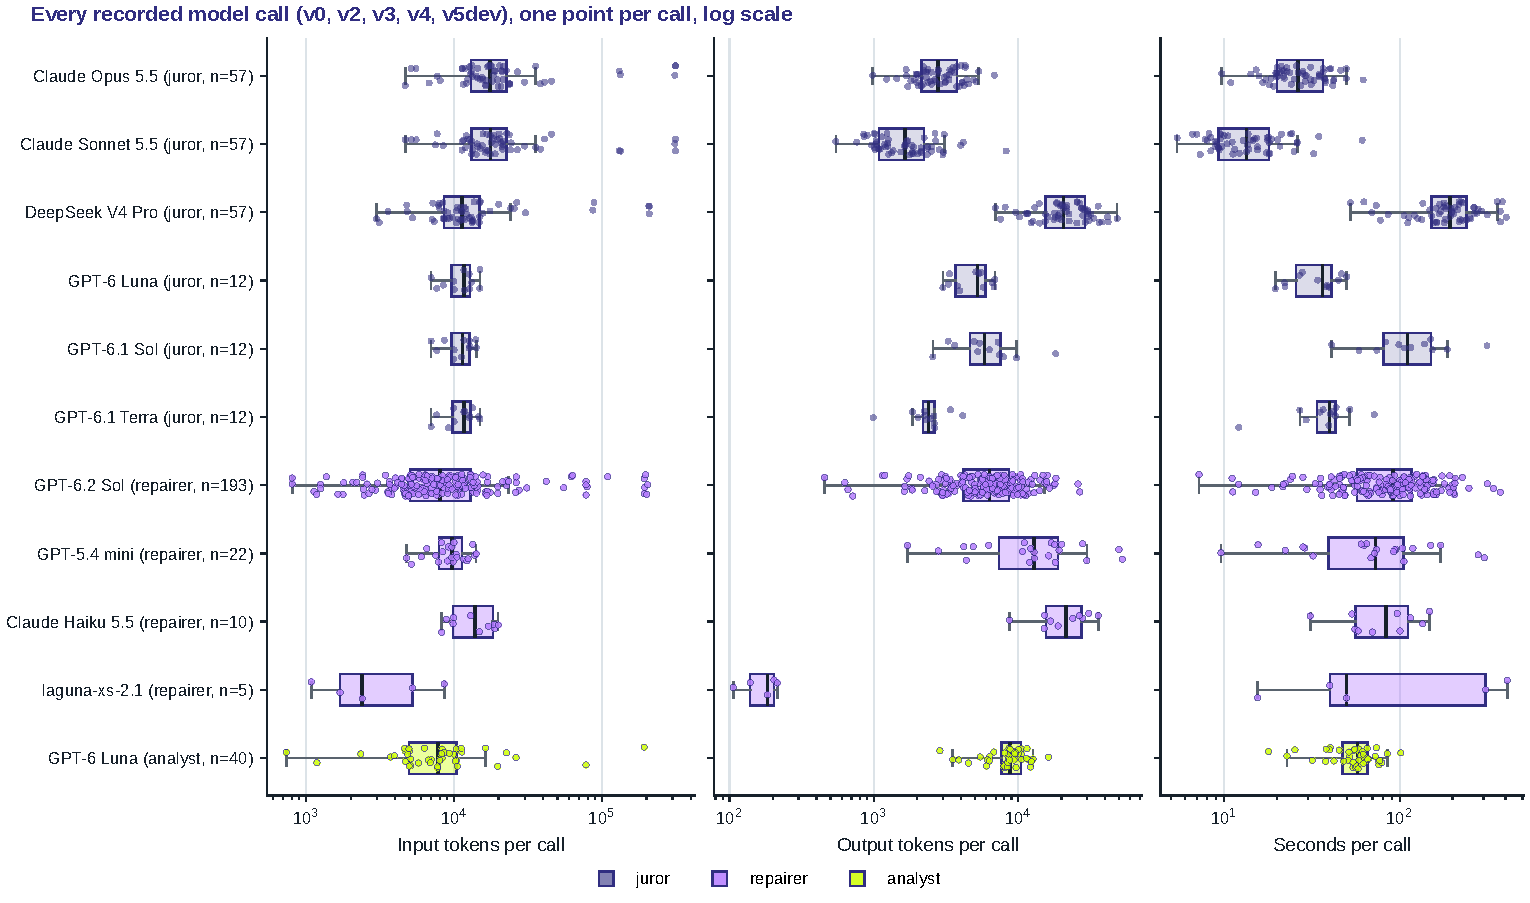
\includegraphics[width=\linewidth]{figures/fig_calls_tokens_time.pdf}
\end{adjustwidth}
\caption{Input tokens, output tokens and latency of every recorded call (v0, v2--v4 and the v5 development check), one point per call, by model and role (colour), on log scales; boxes give the quartiles. Drawn by \texttt{results/figures/make\_figures.py} from \texttt{results/logs/calls/*.csv}.\label{fig:calls}}
\end{figure}

\begin{figure}[H]
\begin{adjustwidth}{-\extralength}{0cm}
\centering
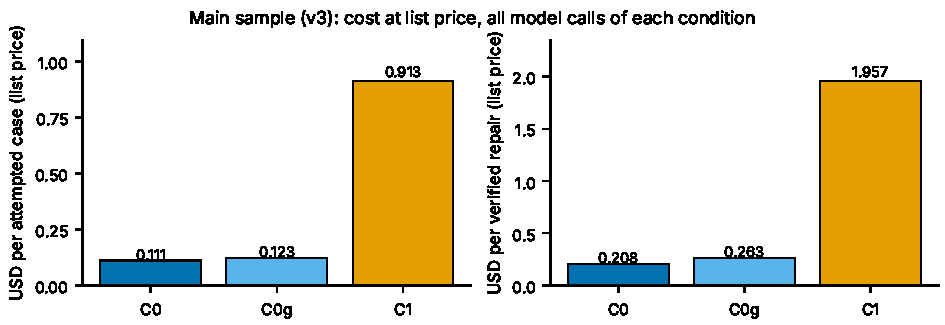
\includegraphics[width=\linewidth]{figures/fig_cost_per_repair.pdf}
\end{adjustwidth}
\caption{Cost at list price per attempted case (left) and per verified repair (right) in the three conditions of the main sample, counting every model call of each condition. Drawn by \texttt{results/figures/make\_figures.py} from \texttt{results/logs/calls/calls\_v3\_main.csv} and \texttt{experiments/v3\_main/results.csv}.\label{fig:cost}}
\end{figure}

%-----------------------------------------------------------------------------------------------
\section{Discussion}\label{sec:discussion}

\subsection{Main Findings}

\textbf{RQ1.} Even with a valid oracle on every case and a strong repairer, positive repair claims were often false: 42.9\% on the main sample and 65.6\% on the 63 confirmation cases, while 55.2\% and 34.9\% of the repairs were verified. The gap between the two samples shows how much these rates depend on the cases, and the intervals of Table~\ref{tab:main} overlap only partly. The false claims had a common shape: most unverified patches applied and kept the project's functional tests passing, and failed the exploit tests. This is the security counterpart of the plausible but incorrect patches of test-based repair~\cite{Qi2015AnalysisOfPatch,Smith2015IsTheCure}: a patch that looks like a fix and does not break the program, but does not stop the attack.

\textbf{Comparison with the benchmark's own results.} The repairer alone verified 38 of the 92 complete cases of v3 and v4 (41.3\%), whereas the authors of Vul4Py report 4 of 100 for the strongest directly prompted LLM and 41 of 100 for an agentic system~\cite{Bui2026Vul4pyBenchmarkingAutomated}. The context given to the repairer follows their direct-prompting protocol, but the runs are not identical, so the numbers are not compared statistically. Three differences can contribute to the gap and cannot be separated here: the repairer is a newer model; every environment was repaired until the oracle was valid on the machine that ran the experiments, while with the public release only 18 of the 100 cases passed the scan in a sandbox of the same size, and we do not know how many failures in the benchmark's own evaluation came from the environment; and the fixes are public, so newer models are more likely to have seen them during training.

\textbf{RQ2.} Neither the mechanical gate nor the cross-family jury lowered FAR in these samples, although intervals about 35 points wide cannot exclude moderate reductions. The gate checks what can be checked without tests (the patch applies, compiles and changes something), and almost no false claim failed in those ways. The jury had been calibrated, but its calibration set mixed easy candidates (upstream fixes and decoys that change nothing) with real patches, and on the real wrong patches alone the specificity of the Claude jurors was only 0.50--0.60 (\texttt{decisiones\_v2}). The jurors read the same code and hint as the repairer and had no executable evidence, so they shared its blind spot; correlated errors across models are expected~\cite{Kim2025CorrelatedErrorsIn}, and a panel of diverse judges~\cite{Verga2024ReplacingJudgesWith} did not remove them here. Debate and revision added claims rather than removing them: the independent vote of round 0 claimed 21 patches with 9 false, the final unanimous verdict 26 with 12 false, and in the second C1 pilot both wrong patches were accepted only after the debate or the revision. This agrees with the evidence that models rarely correct themselves without external feedback~\cite{Huang2024LargeLanguageModels}, and it qualifies the benefits reported for multi-agent debate on reasoning tasks~\cite{Du2024ImprovingFactualityAnd}. The only rule that lowered FAR, the confident majority, did so by claiming less, and the jury multiplied the cost per verified repair by 9.4.

\textbf{RQ3.} Exploit tests written by a model did not lower FAR either. They were in some cases weaker than the benchmark's exploit tests, since six wrong patches passed them, and in other cases stricter or about something else, since nine correct patches were rejected for bypasses, unblocked attacks or missing evidence. Generated tests helped to detect incorrect patches in test-based repair~\cite{Xiong2018IdentifyingPatchCorrectness}, but tests that must reproduce a vulnerability from a short report are a harder target. The localization rule, in contrast, was confirmed on cases not used to find it: a patch that leaves some hinted line range untouched is more often an incomplete fix, and refusing to claim it removed 29 of 40 false assurances. Two limits keep this from being a general solution. In Vul4Py the hint is the footprint of the upstream fix, so the rule partly measures agreement with the location the maintainers changed; outside the dataset it needs a report with locations (an advisory that names the functions, a scanner finding) and should be expected to be weaker. And it lost 9 of 21 correct claims, so it trades yield for precision, as the confident majority did.

\textbf{RQ4.} The repairer alone was the cheapest configuration of the main sample, at 0.21--0.28~USD per verified repair at list price, and the jury cost 1.96~USD per verified repair without lowering FAR. \pend{v5: whether retrieval raised the VRR of Claude Haiku 5.5 (H1), its FAR, and its cost per verified repair against C0, in two or three sentences}

\subsection{Limitations and Threats to Validity}\label{sec:limits}

\textbf{Oracle.} The installation repairs never changed a test or its expectations, but deselecting tests (in 65 cases by the automatic mechanism, in 26 because the tests asserted the vulnerable behaviour and in 3 because they failed only on the vulnerable version) narrows the functional oracle, so a regression in a deselected test goes unseen. The exploit tests are finite: a patch that passes them may still be exploitable in another way, which would make the true FAR higher, and a test may demand more than the vulnerability requires, which would make it lower. Flaky tests and secrets in the environment cost two cases in v4; v5 adds a rerun for flaky functional tests and a clean environment.

\textbf{Inputs.} Every model received the files that the upstream fix changed and the hinted line ranges, as in Vul4Py's direct-prompting protocol. This makes the task easier than real repair, where the location is unknown, and it ties the coverage rule to the upstream fix. The vulnerabilities and their fixes are public, so models may have seen them during training, and the study cannot separate repair from recall.

\textbf{Samples and statistics.} The main sample has 29 complete cases and the confirmation 63, so most intervals are wide and many comparisons are descriptive; no correction for multiple comparisons was applied to them. The coverage rule was found post hoc and confirmed once, with a power of 0.73 if its true effect equalled the one observed post hoc. The confirmatory analysis was first run before three verdicts were in, against the decisions file; it was rerun at the end with the same conclusion.

\textbf{Models and costs.} One model family repaired in v2--v4, and the results are tied to the model versions available in November 2026. Claude models were used through the subscription client in fresh sessions without tools, which may behave differently from API calls, and the verdicts of a juror varied between calibration runs (\texttt{decisiones\_v2}). Costs are list prices computed from tokens, not billed amounts; DeepSeek prices are peak-hour prices.

\subsection{Next Steps}\label{sec:v6}

The rule fixed before v5 decides what follows. If H1 is confirmed, v6 moves to an n8n workflow (Figure~\ref{fig:v6}) with two parts: environment automation, in which a failing oracle control retrieves similar repairs from the 91 override files and their notes, the 14 test overrides and the two new failures of v4, a cheap model proposes an override, and the override is accepted only if the control becomes healthy without excluding more than 10\% of the functional tests or any exploit test; and the repair with retrieval as a visual workflow. If H1 is not confirmed, the retrieval step is tuned on the five development cases first, and any new measurement on the 95 cases is reported as exploratory, since Vul4Py has no unused cases left. Independently of v5, the coverage rule should be tested with locations taken from advisories rather than from the upstream fix, and with repairers from other families.

\begin{figure}[H]
\begin{adjustwidth}{-\extralength}{0cm}
\centering
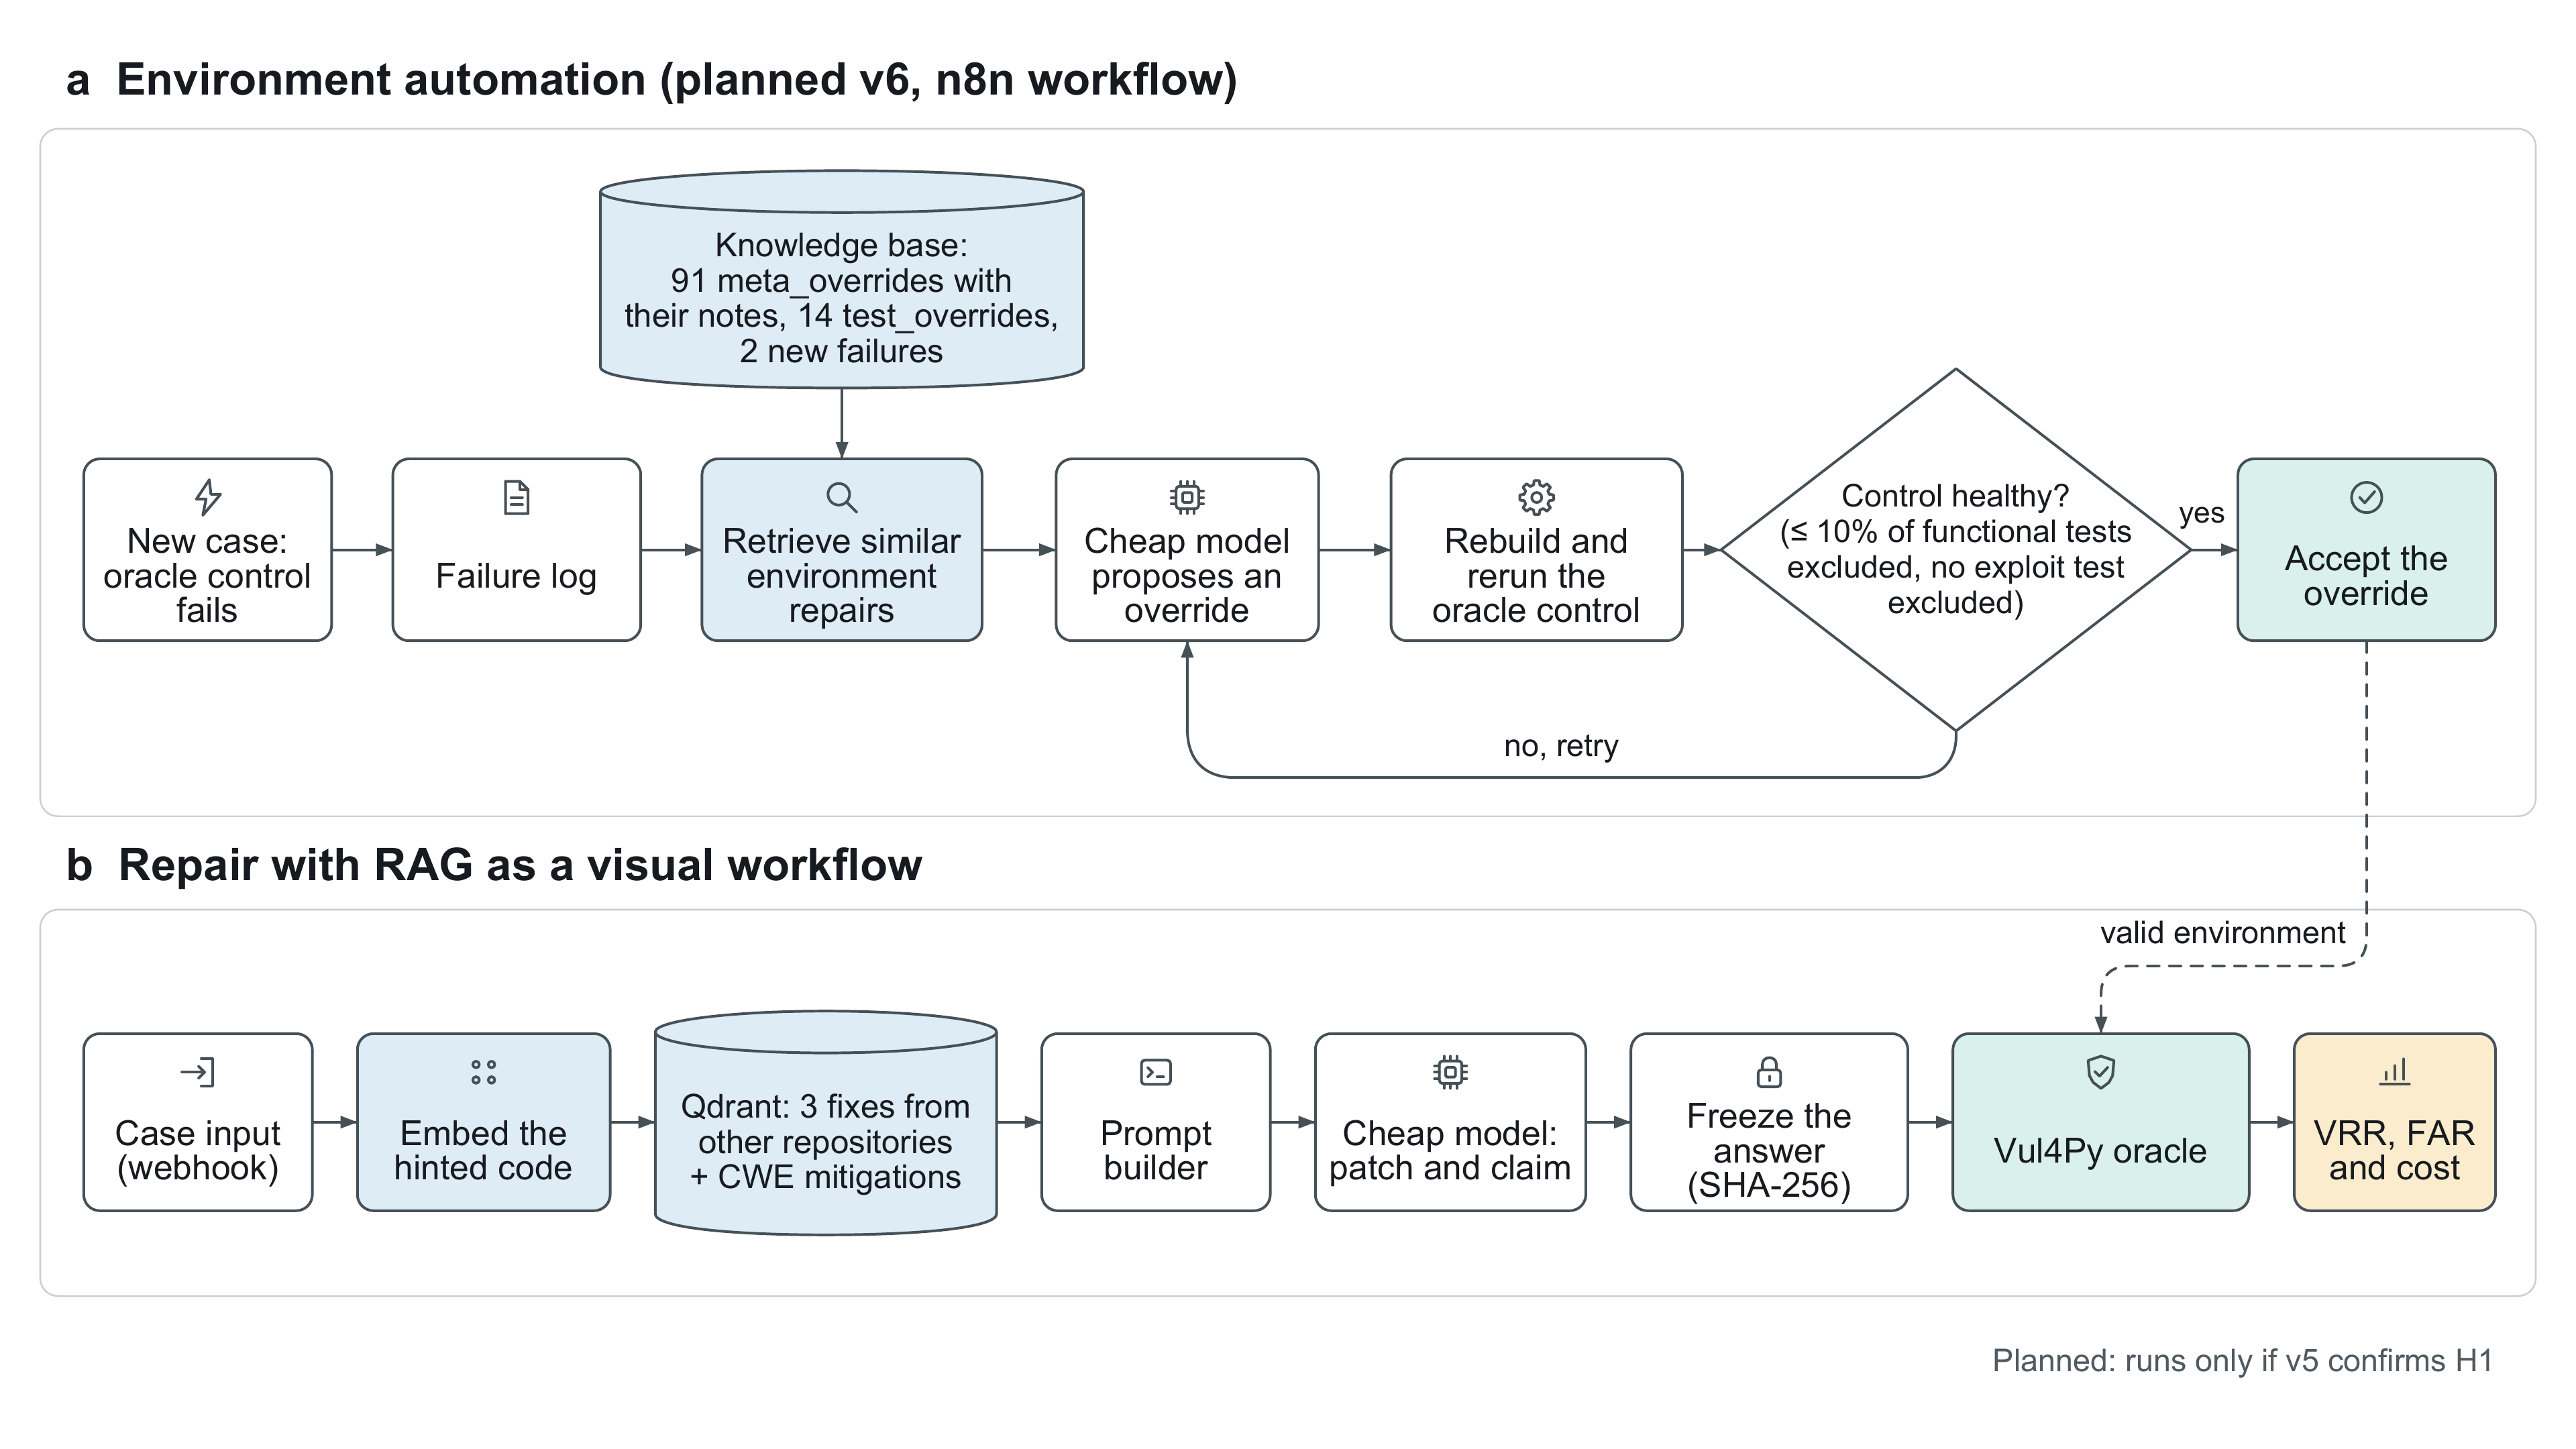
\includegraphics[width=\linewidth]{figures/fig_v6_workflow_chatgpt.png}
\end{adjustwidth}
\caption{Planned v6, from the rule fixed in \texttt{decisiones\_v5}: (\textbf{a}) automatic environment repair with retrieval over the recorded overrides; (\textbf{b}) the repair with retrieval as a visual workflow. It runs only if v5 confirms H1, and it will have its own decisions file, which may change details such as the number of retries. Drawn with ChatGPT (OpenAI) from a prompt that listed every component, label and connection (Section~\ref{sec:ai}).\label{fig:v6}}
\end{figure}

%-----------------------------------------------------------------------------------------------
\section{Conclusions}\label{sec:conclusions}

On Vul4Py with a valid oracle on all 100 cases, 43--66\% of the positive repair claims of a strong LLM were false, and most false claims came with patches that kept the functional tests passing and the exploit tests failing. In these samples, verification by models, whether a mechanical gate, a calibrated cross-family jury with debate and revision, or exploit tests written by a model, did not lower the false assurance rate, and the jury multiplied the cost per verified repair by 9.4. A simple localization rule did lower it, confirmed on 63 unused cases, at the price of 9 of 21 correct claims and with a hint that comes from the upstream fix. \pend{v5: one sentence on retrieval for the cheaper model} Claims about a repair should therefore be backed by executable evidence of the kind the oracle uses, and the cost of every verification step should be reported with its effect.

\vspace{6pt}

\authorcontributions{C.V. designed the study, built and validated the environments, ran the experiments, analysed the data and wrote the manuscript.}

\funding{This research received no external funding.}

\institutionalreview{Not applicable.}

\informedconsent{Not applicable.}

\dataavailability{The decisions files, case lists, results tables, per-call logs, console logs, environment repairs, scripts and figure code are available in the project repository (\url{https://github.com/Camimilo-11/Ai-Yachay-2026/tree/main/Project-Vul4py}), with one folder per version under \texttt{experiments/}. For v0 and for every case of v2--v4 and the v5 development check that went through the pipeline, these folders also hold the answers of every model, the patches, the oracle's evaluation and the frozen record of every call with the SHA-256 of its prompt; the prompts of v2--v5 are rebuilt from the benchmark and are not included. The prepared workspaces (about 100~GB) are not included; every result comes with the command that produced it. No API keys are included.}

\acknowledgments{The author thanks Eugenio Morocho for approving the use of NVIDIA's API catalog for the pilot. The OpenAI and DeepSeek API credit used in v2--v4 was provided for the course. During the preparation of this study and manuscript, the author used Claude Opus 5.5 (Anthropic) to write and review analysis code, organise the repository, write the TikZ code of two diagrams and the prompts of two others, and draft and edit the manuscript, and ChatGPT (OpenAI, model GPT-6.2 Sol) to draw Figures~\ref{fig:v5} and~\ref{fig:v6}, as described in Section~\ref{sec:ai}. The author has reviewed and edited the output and takes full responsibility for the content of this publication.}

\conflictsofinterest{The author declares no conflicts of interest.}

\abbreviations{Abbreviations}{
The following abbreviations are used in this manuscript:\\
\noindent
\begin{tabular}{@{}ll}
API & Application programming interface \\
AUROC & Area under the receiver operating characteristic curve \\
CI & Confidence interval \\
CVE & Common Vulnerabilities and Exposures \\
CWE & Common Weakness Enumeration \\
FAR & False assurance rate \\
LLM & Large language model \\
RAG & Retrieval-augmented generation \\
RQ & Research question \\
VRR & Verified repair rate \\
\end{tabular}
}

\begin{adjustwidth}{-\extralength}{0cm}
\reftitle{References}
\bibliography{references}
\PublishersNote{}
\end{adjustwidth}

\end{document}
